% Options for packages loaded elsewhere
\PassOptionsToPackage{unicode}{hyperref}
\PassOptionsToPackage{hyphens}{url}
\documentclass[
  11pt,
]{article}
\usepackage{xcolor}
\usepackage[margin=2.5cm]{geometry}
\usepackage{amsmath,amssymb}
\setcounter{secnumdepth}{-\maxdimen} % remove section numbering
\usepackage{iftex}
\ifPDFTeX
  \usepackage[T1]{fontenc}
  \usepackage[utf8]{inputenc}
  \usepackage{textcomp} % provide euro and other symbols
\else % if luatex or xetex
  \usepackage{unicode-math} % this also loads fontspec
  \defaultfontfeatures{Scale=MatchLowercase}
  \defaultfontfeatures[\rmfamily]{Ligatures=TeX,Scale=1}
\fi
\usepackage{lmodern}
\ifPDFTeX\else
  % xetex/luatex font selection
\fi
% Use upquote if available, for straight quotes in verbatim environments
\IfFileExists{upquote.sty}{\usepackage{upquote}}{}
\IfFileExists{microtype.sty}{% use microtype if available
  \usepackage[]{microtype}
  \UseMicrotypeSet[protrusion]{basicmath} % disable protrusion for tt fonts
}{}
\usepackage{setspace}
\makeatletter
\@ifundefined{KOMAClassName}{% if non-KOMA class
  \IfFileExists{parskip.sty}{%
    \usepackage{parskip}
  }{% else
    \setlength{\parindent}{0pt}
    \setlength{\parskip}{6pt plus 2pt minus 1pt}}
}{% if KOMA class
  \KOMAoptions{parskip=half}}
\makeatother
\usepackage{longtable,booktabs,array}
\newcounter{none} % for unnumbered tables
\usepackage{calc} % for calculating minipage widths
% Correct order of tables after \paragraph or \subparagraph
\usepackage{etoolbox}
\makeatletter
\patchcmd\longtable{\par}{\if@noskipsec\mbox{}\fi\par}{}{}
\makeatother
% Allow footnotes in longtable head/foot
\IfFileExists{footnotehyper.sty}{\usepackage{footnotehyper}}{\usepackage{footnote}}
\makesavenoteenv{longtable}
\usepackage{graphicx}
\makeatletter
\newsavebox\pandoc@box
\newcommand*\pandocbounded[1]{% scales image to fit in text height/width
  \sbox\pandoc@box{#1}%
  \Gscale@div\@tempa{\textheight}{\dimexpr\ht\pandoc@box+\dp\pandoc@box\relax}%
  \Gscale@div\@tempb{\linewidth}{\wd\pandoc@box}%
  \ifdim\@tempb\p@<\@tempa\p@\let\@tempa\@tempb\fi% select the smaller of both
  \ifdim\@tempa\p@<\p@\scalebox{\@tempa}{\usebox\pandoc@box}%
  \else\usebox{\pandoc@box}%
  \fi%
}
% Set default figure placement to htbp
\def\fps@figure{htbp}
\makeatother
% definitions for citeproc citations
\NewDocumentCommand\citeproctext{}{}
\NewDocumentCommand\citeproc{mm}{%
  \begingroup\def\citeproctext{#2}\cite{#1}\endgroup}
\makeatletter
 % allow citations to break across lines
 \let\@cite@ofmt\@firstofone
 % avoid brackets around text for \cite:
 \def\@biblabel#1{}
 \def\@cite#1#2{{#1\if@tempswa , #2\fi}}
\makeatother
\newlength{\cslhangindent}
\setlength{\cslhangindent}{1.5em}
\newlength{\csllabelwidth}
\setlength{\csllabelwidth}{3em}
\newenvironment{CSLReferences}[2] % #1 hanging-indent, #2 entry-spacing
 {\begin{list}{}{%
  \setlength{\itemindent}{0pt}
  \setlength{\leftmargin}{0pt}
  \setlength{\parsep}{0pt}
  % turn on hanging indent if param 1 is 1
  \ifodd #1
   \setlength{\leftmargin}{\cslhangindent}
   \setlength{\itemindent}{-1\cslhangindent}
  \fi
  % set entry spacing
  \setlength{\itemsep}{#2\baselineskip}}}
 {\end{list}}
\usepackage{calc}
\newcommand{\CSLBlock}[1]{\hfill\break\parbox[t]{\linewidth}{\strut\ignorespaces#1\strut}}
\newcommand{\CSLLeftMargin}[1]{\parbox[t]{\csllabelwidth}{\strut#1\strut}}
\newcommand{\CSLRightInline}[1]{\parbox[t]{\linewidth - \csllabelwidth}{\strut#1\strut}}
\newcommand{\CSLIndent}[1]{\hspace{\cslhangindent}#1}
\setlength{\emergencystretch}{3em} % prevent overfull lines
\providecommand{\tightlist}{%
  \setlength{\itemsep}{0pt}\setlength{\parskip}{0pt}}
\usepackage{amsmath}
\usepackage{amssymb}
\usepackage{bookmark}
\IfFileExists{xurl.sty}{\usepackage{xurl}}{} % add URL line breaks if available
\urlstyle{same}
% fallback for those not using the hyperref driver hyperxmp:
\makeatletter
\@ifundefined{xmpquote}{\newcommand{\xmpquote}[1]{#1}}{}
\makeatother
\hypersetup{
  pdftitle={IGNITE: Automatisierte{,} deterministische Thermografie-Pipeline zur Früherkennung pathologischer Entzündungsherde im klinischen Arbeitsumfeld},
  pdfauthor={Jona Noack},
  hidelinks,
  pdfcreator={LaTeX via pandoc}}

\title{IGNITE: Automatisierte, deterministische Thermografie-Pipeline
zur Früherkennung pathologischer Entzündungsherde im klinischen
Arbeitsumfeld}
\author{Jona Noack}
\date{2026-07-23}

\begin{document}
\maketitle

\setstretch{1.5}
\section{Projektüberblick}\label{projektuxfcberblick}

In diesem Projekt für den Wettbewerb \emph{Jugend forscht 2026}
(Fachgebiet Arbeitswelt) wird die Software \textbf{IGNITE} vorgestellt.
Die Arbeit untersucht Möglichkeiten zur Automatisierung der
thermografischen Entzündungserkennung im medizinischen
Behandlungsalltag. Bisher müssen Ärztinnen, Ärzte und Podologen
Wärmebildaufnahmen von Risikopatienten -- beispielsweise beim
diabetischen Fußsyndrom -- manuell am Bildschirm auswerten. Diese
visuelle Sichtprüfung erfordert viel Zeit (ca. 3 bis 5 Minuten pro
Aufnahme), ist subjektiv und unterliegt tageszeitlichen
Ermüdungsfaktoren des Personals.

Die entwickelte Software nutzt eine 5-stufige mathematische
Bildverarbeitungs-Pipeline, um physiologische Temperaturverläufe zu
filtern, Störabstrahlungen des Raumes zu erodieren und lokale
Hitzespitzen als potenzielle Entzündungsherde zu isolieren. Um
Verzögerungen im Praxisablauf zu vermeiden, wurde der Rechenkern in der
Programmiersprache Rust umgesetzt und mittels Rayon parallelisiert,
wodurch Auswertungszeiten unter 30 Millisekunden erreicht werden. Ein
integrierter Instant-Splash-Screen startet die Benutzeroberfläche in
unter 50 Millisekunden.

Auf synthetischen Datensätzen mit simulierten Rauschmodellen erzielte
das System eine Sensitivität von 1,00 sowie einen Dice-Koeffizienten von
0,88 bis 0,91. Bei 21 realen klinischen Testaufnahmen wurden auffällige
Stellen zuverlässig abgegrenzt. Die Arbeit analysiert jedoch auch die
deutlichen Grenzen des Verfahrens: Da ein deterministischer Filter nicht
zwischen biologischen Infektionen und harmlosen mechanischen
Druckstellen (z. B. durch Socken oder Gehlenken) unterscheiden kann,
stellt die Software kein Medizinprodukt dar, sondern dient als
Orientierungshilfe unter ärztlicher Aufsicht.

\begin{center}\rule{0.5\linewidth}{0.5pt}\end{center}

\section{Inhaltsverzeichnis}\label{inhaltsverzeichnis}

\begin{enumerate}
\def\labelenumi{\arabic{enumi}.}
\tightlist
\item
  \hyperref[1-einleitung-und-problemstellung]{Einleitung und
  Problemstellung}

  \begin{itemize}
  \tightlist
  \item
    1.1 Belastungssituation im medizinischen Behandlungsalltag
  \item
    1.2 Relevanz der Früherkennung beim Diabetischen Fußsyndrom
  \item
    1.3 Zielsetzung und Forschungsfragen
  \end{itemize}
\item
  \hyperref[2-hintergrund-und-theoretische-grundlagen]{Hintergrund und
  theoretische Grundlagen}

  \begin{itemize}
  \tightlist
  \item
    2.1 Medizintechnischer Kontext und podiatrischer Goldstandard
  \item
    2.2 Physikalische Radiometrie und Strahlungsmodell
  \item
    2.3 Kritische Vergleichsmatrix bestehender Auswerteverfahren
  \item
    2.4 Mathematische Ausarbeitung der 5-Stufen-Pipeline
  \end{itemize}
\item
  \hyperref[3-vorgehensweise-materialien-und-methoden]{Vorgehensweise,
  Materialien und Methoden}

  \begin{itemize}
  \tightlist
  \item
    3.1 Analyse und Ergonomie des klinischen Behandlungsablaufs
  \item
    3.2 Software-Architektur und Multi-Backend-Konzept
  \item
    3.3 Schritt-für-Schritt Implementierung in Rust
  \item
    3.4 Ergonomische Benutzeroberfläche und Instant-Splash-UX
  \item
    3.5 Datenschutzkonzept im Arbeitsumfeld
  \item
    3.6 Selbstständig erbrachter Projektanteil
  \end{itemize}
\item
  \hyperref[4-bildgestuxfctzte-visualisierung-der-pipeline-stufen]{Bildgestützte
  Visualisierung der Pipeline-Stufen}

  \begin{itemize}
  \tightlist
  \item
    4.1 Ausgangsmaterial (Original-Thermogramm)
  \item
    4.2 Körpermaskierung und Distanzkarte (Stufe 2)
  \item
    4.3 Hintergrundkorrektur via Top-Hat-Transformation (Stufe 3)
  \item
    4.4 Statistisches Thresholding und Hotspot-Maske (Stufe 4 \& 5)
  \item
    4.5 Finales diagnostisches Overlay für das Behandlungszimmer
  \item
    4.6 Auswertung synthetischer Krankheits-Szenarien
  \end{itemize}
\item
  \hyperref[5-ergebnisse]{Ergebnisse}

  \begin{itemize}
  \tightlist
  \item
    5.1 Laufzeitmessungen und Rechenzeiten
  \item
    5.2 Parameter-Sensitivitätsanalyse des Schwellenwert-Faktors k
  \item
    5.3 Quantitativer Benchmark auf synthetischen Entzündungsszenarien
  \item
    5.4 Auswertung auf 21 realen klinischen Testbildern
  \item
    5.5 Mathematische Backend-Paritätstests
  \end{itemize}
\item
  \hyperref[6-ergebnisdiskussion-und-kritische-wuxfcrdigung]{Ergebnisdiskussion
  und Kritische Würdigung}

  \begin{itemize}
  \tightlist
  \item
    6.1 Einordnung der Ergebnisse bezüglich der Arbeitserleichterung
  \item
    6.2 Überprüfung der Hypothesen und Bedeutung von Robust-MAD
  \item
    6.3 Ausführliche Analyse der Nachteile, Grenzen und Störfaktoren
  \end{itemize}
\item
  \hyperref[7-fazit-und-ausblick]{Fazit und Ausblick}

  \begin{itemize}
  \tightlist
  \item
    7.1 Gesamtfazit zur Arbeitswelt-Fragestellung
  \item
    7.2 Zukünftige Erweiterungen für den Praxiseinsatz
  \end{itemize}
\item
  \hyperref[8-literaturverzeichnis]{Literaturverzeichnis}
\item
  \hyperref[9-unterstuxfctzungsleistungen]{Unterstützungsleistungen}
\end{enumerate}

\begin{center}\rule{0.5\linewidth}{0.5pt}\end{center}

\section{1. Einleitung und
Problemstellung}\label{einleitung-und-problemstellung}

\subsection{1.1 Belastungssituation im medizinischen
Behandlungsalltag}\label{belastungssituation-im-medizinischen-behandlungsalltag}

Die demografische Entwicklung und die Zunahme chronischer
Stoffwechselerkrankungen stellen das medizinische Fachpersonal in Praxen
und Kliniken vor erhebliche kapazitäre Herausforderungen (Ring and Ammer
2012). Insbesondere in der Podiatrie, Diabetologie und Dermatologie
müssen täglich zahlreiche Risikopatienten untersucht werden.

Das manuelle Durchmustern von Wärmebildaufnahmen zur Identifikation
pathologischer Hitzespitzen erfordert konzentriertes Absuchen am
Bildschirm, das manuelle Einstellen dynamischer Farbskalen sowie das
Ausmessen kontralateraler Temperaturdifferenzen. Für eine qualifizierte
Erstbeurteilung einer thermografischen Aufnahme benötigt eine Fachkraft
im Schnitt 3 bis 5 Minuten (Müller 2022). Bei einer Tagesfrequenz von 20
bis 30 Patienten summiert sich dieser Zusatzaufwand zu einer Arbeitszeit
von über 1,5 Stunden, die für das persönliche Arzt-Patienten-Gespräch
fehlt.

Darüber hinaus birgt die rein visuelle Sichtprüfung ein relevantes
Fehlerrisiko: Die wahrgenommene Intensität einer Entzündungszone auf
Farbskalen (z. B. \emph{Rainbow}- oder \emph{Jet}-Colormaps) hängt stark
von der individuellen Farbkontrasteinstellung des Monitors sowie von
Ermüdungsfaktoren des Fachpersonals am Ende einer Schicht ab.

\subsection{1.2 Relevanz der Früherkennung beim Diabetischen
Fußsyndrom}\label{relevanz-der-fruxfcherkennung-beim-diabetischen-fuuxdfsyndrom}

Das diabetische Fußsyndrom (DFS) ist eine Folgeerscheinung der distalen
sensomotorischen Polyneuropathie und der peripheren arteriellen
Verschlusskrankheit (pAVK). Wegen des Verlusts des Protektivempfindens
bleiben biomechanische Überlastungen, Mikrotraumen oder Druckstellen vom
Patienten unbemerkt (Armstrong et al. 2007).

Entzündliche Prozesse im tiefen Gewebe führen durch Hyperämie und
gesteigerte Stoffwechselaktivität zu lokal abgegrenzten
Temperaturerhöhungen der Hautoberfläche. Diese thermischen Anomalien
treten häufig Tage bis Wochen auf, bevor histologische Gewebedefekte
oder ulzeröse Hautdurchbrüche sichtbar werden. Eine verlässliche
Früherkennung ermöglicht frühzeitige Entlastungsmaßnahmen (z. B.
orthopädische Schuhanpassungen) und kann das Risiko von
Unterschenkelamputationen maßgeblich senken (Armstrong et al. 2007).

\subsection{1.3 Zielsetzung und
Forschungsfragen}\label{zielsetzung-und-forschungsfragen}

Ziel dieser Arbeit ist die Konzeption, Implementierung und mathematische
Validierung von \textbf{IGNITE}, einer hochperformanten, lokal
auszuführenden Software zur automatisierten Hotspot-Isolierung. Das
System soll das Fachpersonal durch eine objektive visuelle
Orientierungshilfe entlasten, ohne den klinischen Behandlungsfluss durch
Ladezeiten zu hemmen.

Folgende Forschungsfragen stehen im Zentrum der Untersuchung: *
\textbf{Forschungsfrage 1 (Arbeitserleichterung \& Erklärbarkeit):}
Lässt sich ein deterministischer, mathematisch vollständig
nachvollziehbarer Algorithmus entwickeln, der Entzündungsareale auf
synthetischen Testdaten mit einer Sensitivität von \(> 0{,}95\)
markiert, ohne auf undurchsichtige KI-Blackbox-Modelle zurückzufragen? *
\textbf{Forschungsfrage 2 (Geschwindigkeit \& Ergonomie):} Kann durch
die Implementierung in nativem Rust mit Multi-Threading eine Rechenzeit
von \(< 50\text{ ms}\) realisiert werden, sodass die Auswertung im
Behandlungszimmer verzögerungsfrei erfolgt? * \textbf{Forschungsfrage 3
(Kritische Grenzen):} Wo liegen die physikalischen und algorithmischen
Schwachstellen eines rein Schwellenwert-basierten Verfahrens im realen
Praxisbetrieb?

\begin{center}\rule{0.5\linewidth}{0.5pt}\end{center}

\section{2. Hintergrund und theoretische
Grundlagen}\label{hintergrund-und-theoretische-grundlagen}

\subsection{2.1 Medizintechnischer Kontext und podiatrischer
Goldstandard}\label{medizintechnischer-kontext-und-podiatrischer-goldstandard}

In der medizinischen Thermografie gilt die vergleichende Analyse
symmetrischer Körperareale (kontralaterale Asymmetrie) als
diagnostischer Goldstandard (Armstrong et al. 2007; Ring and Ammer
2012). Da die physiologische Hauttemperatur systemischen Schwankungen
(z. B. Zirkadianer Rhythmus, Raumtemperatur) unterliegt, ist der
absolute Temperaturwert einzelner Pixel nur bedingt aussagekräftig.

Eine kontralaterale Temperaturdifferenz von

\[ \Delta T = |T_{\text{links}} - T_{\text{rechts}}| > 2{,}2\,^\circ\text{C} \]

an anatomisch identischen Messpunkten gilt in der Podiatrie als klinisch
signifikanter Indikator für entzündliche Gewebeprozesse (Armstrong et
al. 2007).

\pandocbounded{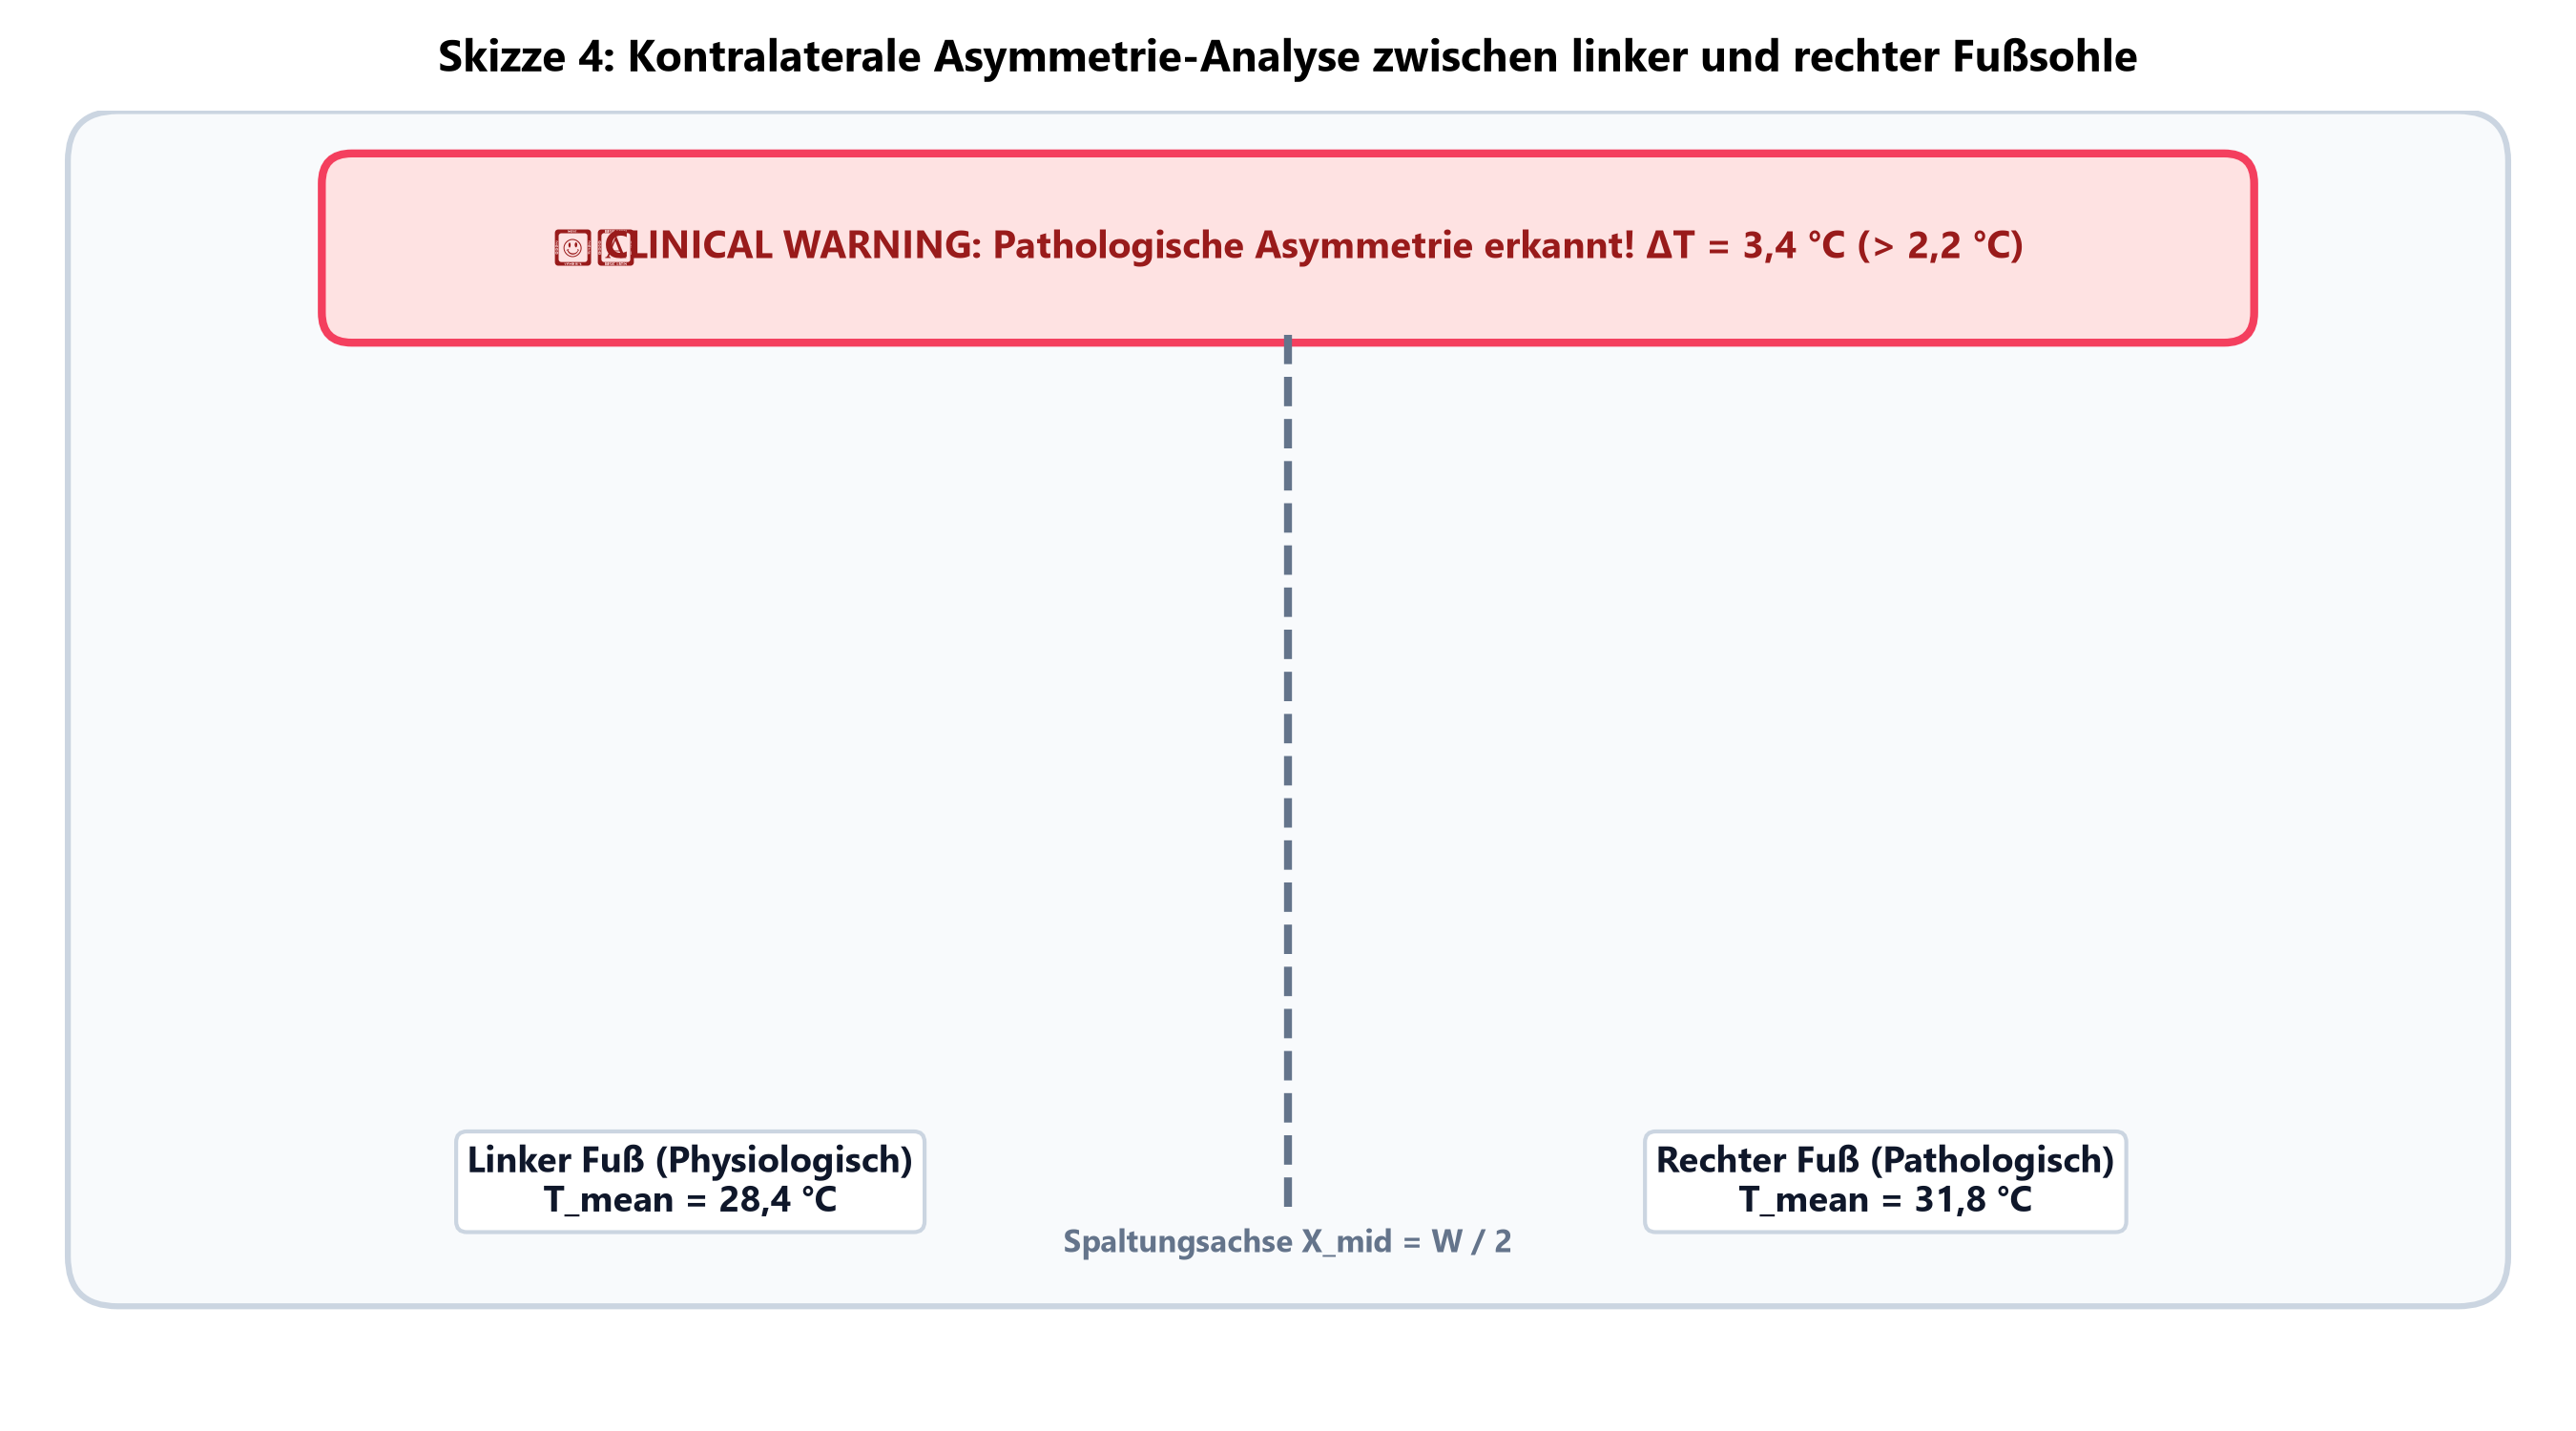
\includegraphics[keepaspectratio,alt={Skizze 4: Kontralaterale Asymmetrie-Analyse}]{images/skizze_asymmetrie_analyse.png}}\\
\emph{Abbildung 1 (Skizze 4): Prinzip der kontralateralen
Asymmetrie-Analyse in der Podiatrie. Das Bild wird an der Bildmitte
getrennt, um die mittleren Oberflächentemperaturen beider Fußsohlen zu
vergleichen. Bei einer Abweichung von
\(\Delta T > 2{,}2\,^\circ\text{C}\) erscheint ein Warnhinweis.}

\begin{center}\rule{0.5\linewidth}{0.5pt}\end{center}

\subsection{2.2 Physikalische Radiometrie und
Strahlungsmodell}\label{physikalische-radiometrie-und-strahlungsmodell}

Die Infrarot-Thermografie basiert auf dem Stefan-Boltzmann-Gesetz
(Stefan 1879; Boltzmann 1884), das die spezifische Ausstrahlung \(M\)
eines schwarzen Körpers in Abhängigkeit von der thermodynamischen
Temperatur \(T\) beschreibt:

\[ M = \sigma \cdot T^4 \]

wobei
\(\sigma \approx 5{,}670374 \times 10^{-8}\,\text{W}\,\text{m}^{-2}\,\text{K}^{-4}\)
die Stefan-Boltzmann-Konstante bezeichnet. Für reale Körper mit dem
spezifischen Emissivitätsgrad \(\epsilon \in (0, 1)\) und unter
Berücksichtigung der von der Umgebung reflektierten Infrarotstrahlung
\(T_{\text{refl}}\) gilt für die vom Sensor erfasste Gewebetemperature
\(T_{\text{obj}}\) (Müller 2022):

\[ T_{\text{obj}} = \left( \frac{T_{\text{meas}}^4 - (1 - \epsilon) \cdot T_{\text{refl}}^4}{\epsilon} \right)^{1/4} \]

Für menschliche Hautgewebe gilt in der medizinischen Praxis der
Literaturwert \(\epsilon \approx 0{,}98\) (Ring and Ammer 2012).
Infrarotkameras transformieren das thermische Strahlungsfeld in eine
8-Bit-Grauwertmatrix \(I(x,y) \in [0, 255]\), deren Intensität linear
mit dem eingestellten Temperaturbereich \([T_{\min}, T_{\max}]\)
korreliert.

\begin{center}\rule{0.5\linewidth}{0.5pt}\end{center}

\subsection{2.3 Kritische Vergleichsmatrix bestehender
Auswerteverfahren}\label{kritische-vergleichsmatrix-bestehender-auswerteverfahren}

{\def\LTcaptype{none} % do not increment counter
\begin{longtable}[]{@{}
  >{\raggedright\arraybackslash}p{(\linewidth - 4\tabcolsep) * \real{0.3333}}
  >{\raggedright\arraybackslash}p{(\linewidth - 4\tabcolsep) * \real{0.3333}}
  >{\raggedright\arraybackslash}p{(\linewidth - 4\tabcolsep) * \real{0.3333}}@{}}
\toprule\noalign{}
\begin{minipage}[b]{\linewidth}\raggedright
Auswerteverfahren
\end{minipage} & \begin{minipage}[b]{\linewidth}\raggedright
Vorteile im Arbeitsalltag
\end{minipage} & \begin{minipage}[b]{\linewidth}\raggedright
Nachteile und Schwachstellen
\end{minipage} \\
\midrule\noalign{}
\endhead
\bottomrule\noalign{}
\endlastfoot
\textbf{Manuelle Sichtprüfung (Arzt/Podologe)} & • Erkennt den
klinischen Gesamtzusammenhang• Kann Narben, Druckstellen \& Wunden
unterscheiden• Benötigt keine Zusatzsoftware & • Zeitaufwendig (3--5
Minuten pro Bild)• Subjektiv und abhängig von Erfahrung/Tagesform• Keine
automatische Dokumentation \\
\textbf{Einfache Schwellenwert-Filter (Otsu)} & • Sehr schnell
(\textless{} 10 ms)• Einfach zu programmieren & • Versagt bei normalen
Körper-Temperaturverläufen• Sehr viele Falsch-Positive an kalten
Rändern \\
\textbf{Deep-Learning KI (z. B. U-Net)} & • Kann komplexe Formen und
Bildmuster erkennen• Hohe Genauigkeit bei gutem Training & •
``Black-Box'': Entscheidungen nicht mathematisch erklärbar• Oft
Cloud-Zwang (DSGVO-Problem im Krankenhaus)• Benötigt leistungsfähige
GPUs \\
\textbf{Mein Ansatz (IGNITE)} & • Schnelle Berechnung (\textless{} 30 ms
auf normaler CPU)• 100 \% lokal \& DSGVO-konform (kein Cloud-Upload)•
Mathematisch nachvollziehbar & • Kann \textbf{nicht} zwischen Entzündung
\& Druckstelle unterscheiden• Feste Schwellenwerte passen nicht auf
jeden Hauttyp• Kein zertifiziertes Medizinprodukt \\
\end{longtable}
}

\begin{center}\rule{0.5\linewidth}{0.5pt}\end{center}

\subsection{2.4 Mathematische Funktionsweise der
5-Stufen-Pipeline}\label{mathematische-funktionsweise-der-5-stufen-pipeline}

Die Hotspot-Isolierung in IGNITE basiert auf einer 5-stufigen
Bildverarbeitungs-Pipeline (Stiftung Jugend forscht e. V. 2025):

\subsubsection{Stufe 1: Dynamische
Kernel-Skalierung}\label{stufe-1-dynamische-kernel-skalierung}

Um unabhängig von der Sensorauflösung des verwendeten Kamerasystems
(\(160 \times 120\) bis \(1440 \times 1080\) Pixel) identische
geometrische Filtereffekte zu erzielen, skaliert der Radius des
morphologischen Strukturierungselements \(K\) proportional zur minimalen
Bilddimension:

\[ K_{\text{raw}} = \lfloor \min(W, H) \cdot 0{,}05 \rfloor, \quad K_{\text{odd}} = \max(3, K_{\text{raw}} \mid 1) \]

Die bitweise OR-Verknüpfung (\texttt{raw\ \textbar{}\ 1}) erzwingt eine
ungerade Pixelanzahl und garantiert ein eindeutiges mathematisches
Symmetriezentrum.

\subsubsection{Stufe 2: Adaptive Körper-Segmentierung (Chamfer-L2
Distanzerosion)}\label{stufe-2-adaptive-kuxf6rper-segmentierung-chamfer-l2-distanzerosion}

Zur Abtrennung des kühlen Raumes dient die globale Binarisierung nach
Otsu (Otsu 1979). Bei kontrastarmen Aufnahmen greift ein
Dynamik-Fallback (\(I_{\min} + 0{,}3 \cdot \Delta I\)).

Um Messunsicherheiten an den Geweberändern (Luft-Haut-Übergänge) zu
eliminieren, wird die Chamfer-L2-Distanztransformation angewendet. Pixel
mit einem Abstand \(D(x,y)\) unterhalb der relativen Randschwelle werden
erodiert:

\[ \text{Mask}_{\text{eroded}}(x,y) = \begin{cases} 255, & \text{falls } D(x,y) \ge f_{\text{dist}} \cdot \max_{x',y'} D(x',y') \\ 0, & \text{sonst} \end{cases} \]

\subsubsection{Stufe 3: Morphologische
Top-Hat-Transformation}\label{stufe-3-morphologische-top-hat-transformation}

Zur Elimination physiologischer Helligkeitsverläufe (z. B. der
natürlichen Gewewärme im Fußgewölbe) wird die morphologische
Top-Hat-Transformation verwendet:

\[ \text{TopHat}(I) = I - \gamma_K(I) = I - ((I \ominus K) \oplus K) \]

wobei \(\gamma_K(I)\) das morphologische Opening von \(I\) mit dem
Kernel \(K\) bezeichnet. Im Rust-Core ist die 2D-Operation in zwei
sequentielle 1D-Durchläufe (horizontal und vertikal) nach Lemire (Lemire
2011) zerlegt. Die Komplexität pro Pixel sinkt dadurch von \(O(K^2)\)
auf \(O(K)\).

\pandocbounded{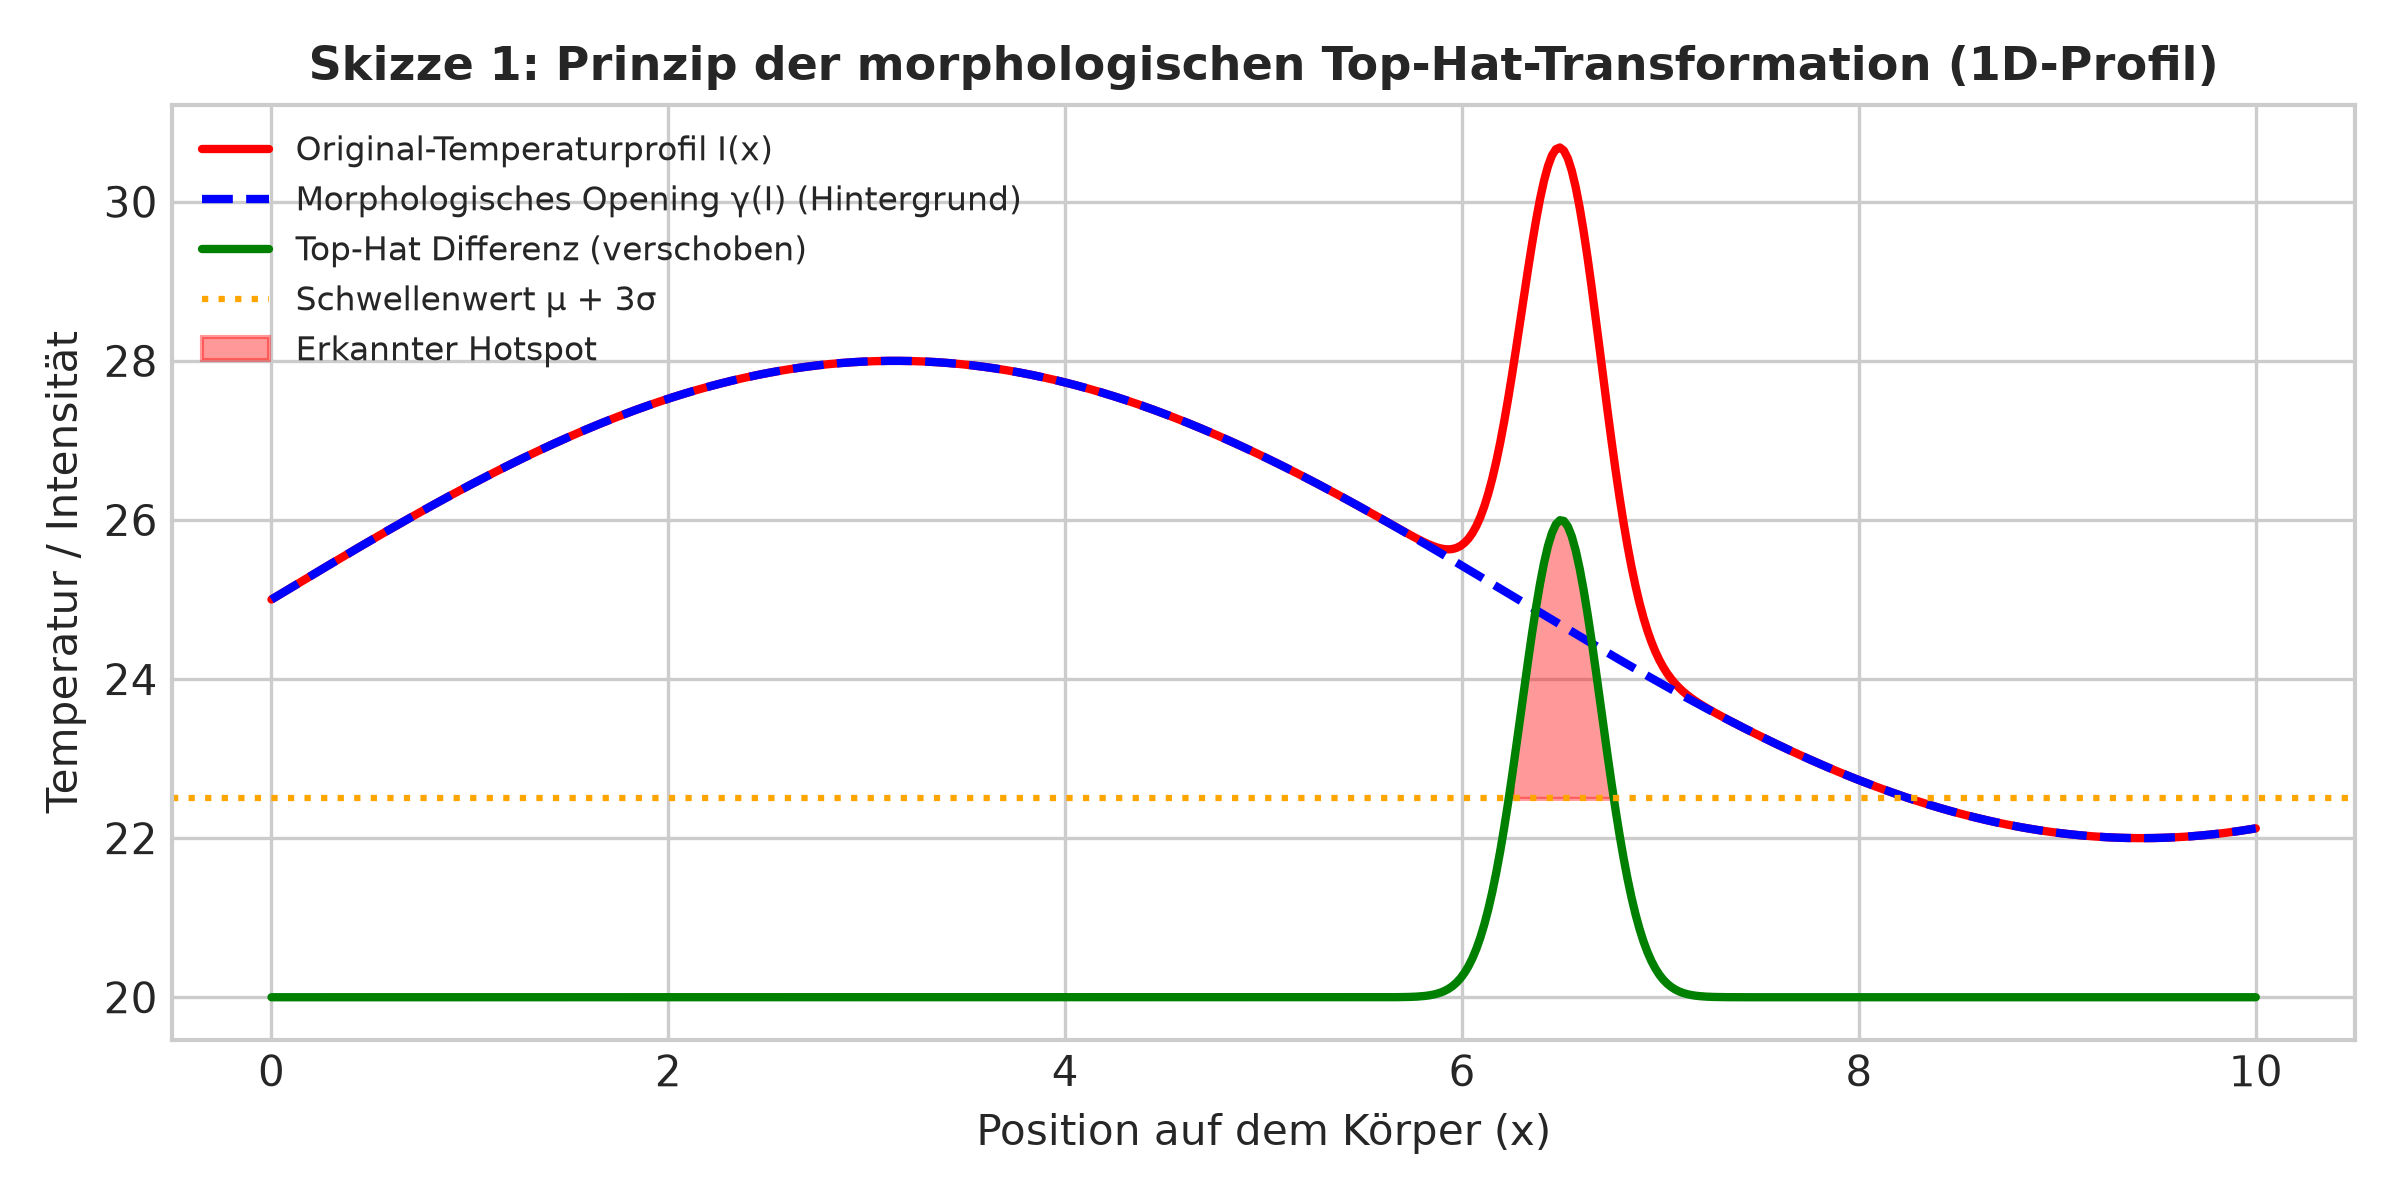
\includegraphics[keepaspectratio,alt={Skizze 1: Prinzip der morphologischen Top-Hat-Transformation}]{images/skizze_tophat_prinzip.png}}\\
\emph{Abbildung 2 (Skizze 1): Das Prinzip der morphologischen
Top-Hat-Transformation im 1D-Temperaturprofil. Das morphologische
Opening glättet großflächige Verläufe. Die Differenz isoliert scharfe
lokale Hitzespitzen oberhalb des Schwellenwerts.}

\begin{center}\rule{0.5\linewidth}{0.5pt}\end{center}

\subsubsection{Stufe 4: Statistisches Outlier-Thresholding (Gauß
vs.~Robust-MAD)}\label{stufe-4-statistisches-outlier-thresholding-gauuxdf-vs.-robust-mad}

Zur Segmentierung signifikanter Hitzespitzen werden zwei statistische
Verfahren unterstützt: 1. \textbf{Gaussian Thresholding:}

\[ T_{\text{Gauß}} = \mu_{\text{diff}} + k \cdot \sigma_{\text{diff}} \]

\begin{enumerate}
\def\labelenumi{\arabic{enumi}.}
\setcounter{enumi}{1}
\tightlist
\item
  \textbf{Robustes MAD-Thresholding:} Bei bimodalen
  Temperaturverteilungen (z. B. stark unterkühlten Zehen) verzerrt der
  kalte Pol den Mittelwert \(\mu\). IGNITE berechnet in diesem Fall die
  robusten Kennzahlen Median (\(\tilde{\mu}\)) und Median Absolute
  Deviation (\(\text{MAD}\)):
\end{enumerate}

\[ \text{MAD} = \text{median}(|X - \tilde{\mu}|), \quad \hat{\sigma}_{\text{MAD}} = 1{,}4826 \cdot \text{MAD} \]

\[ T_{\text{MAD}} = \tilde{\mu} + k \cdot \hat{\sigma}_{\text{MAD}} \]

\pandocbounded{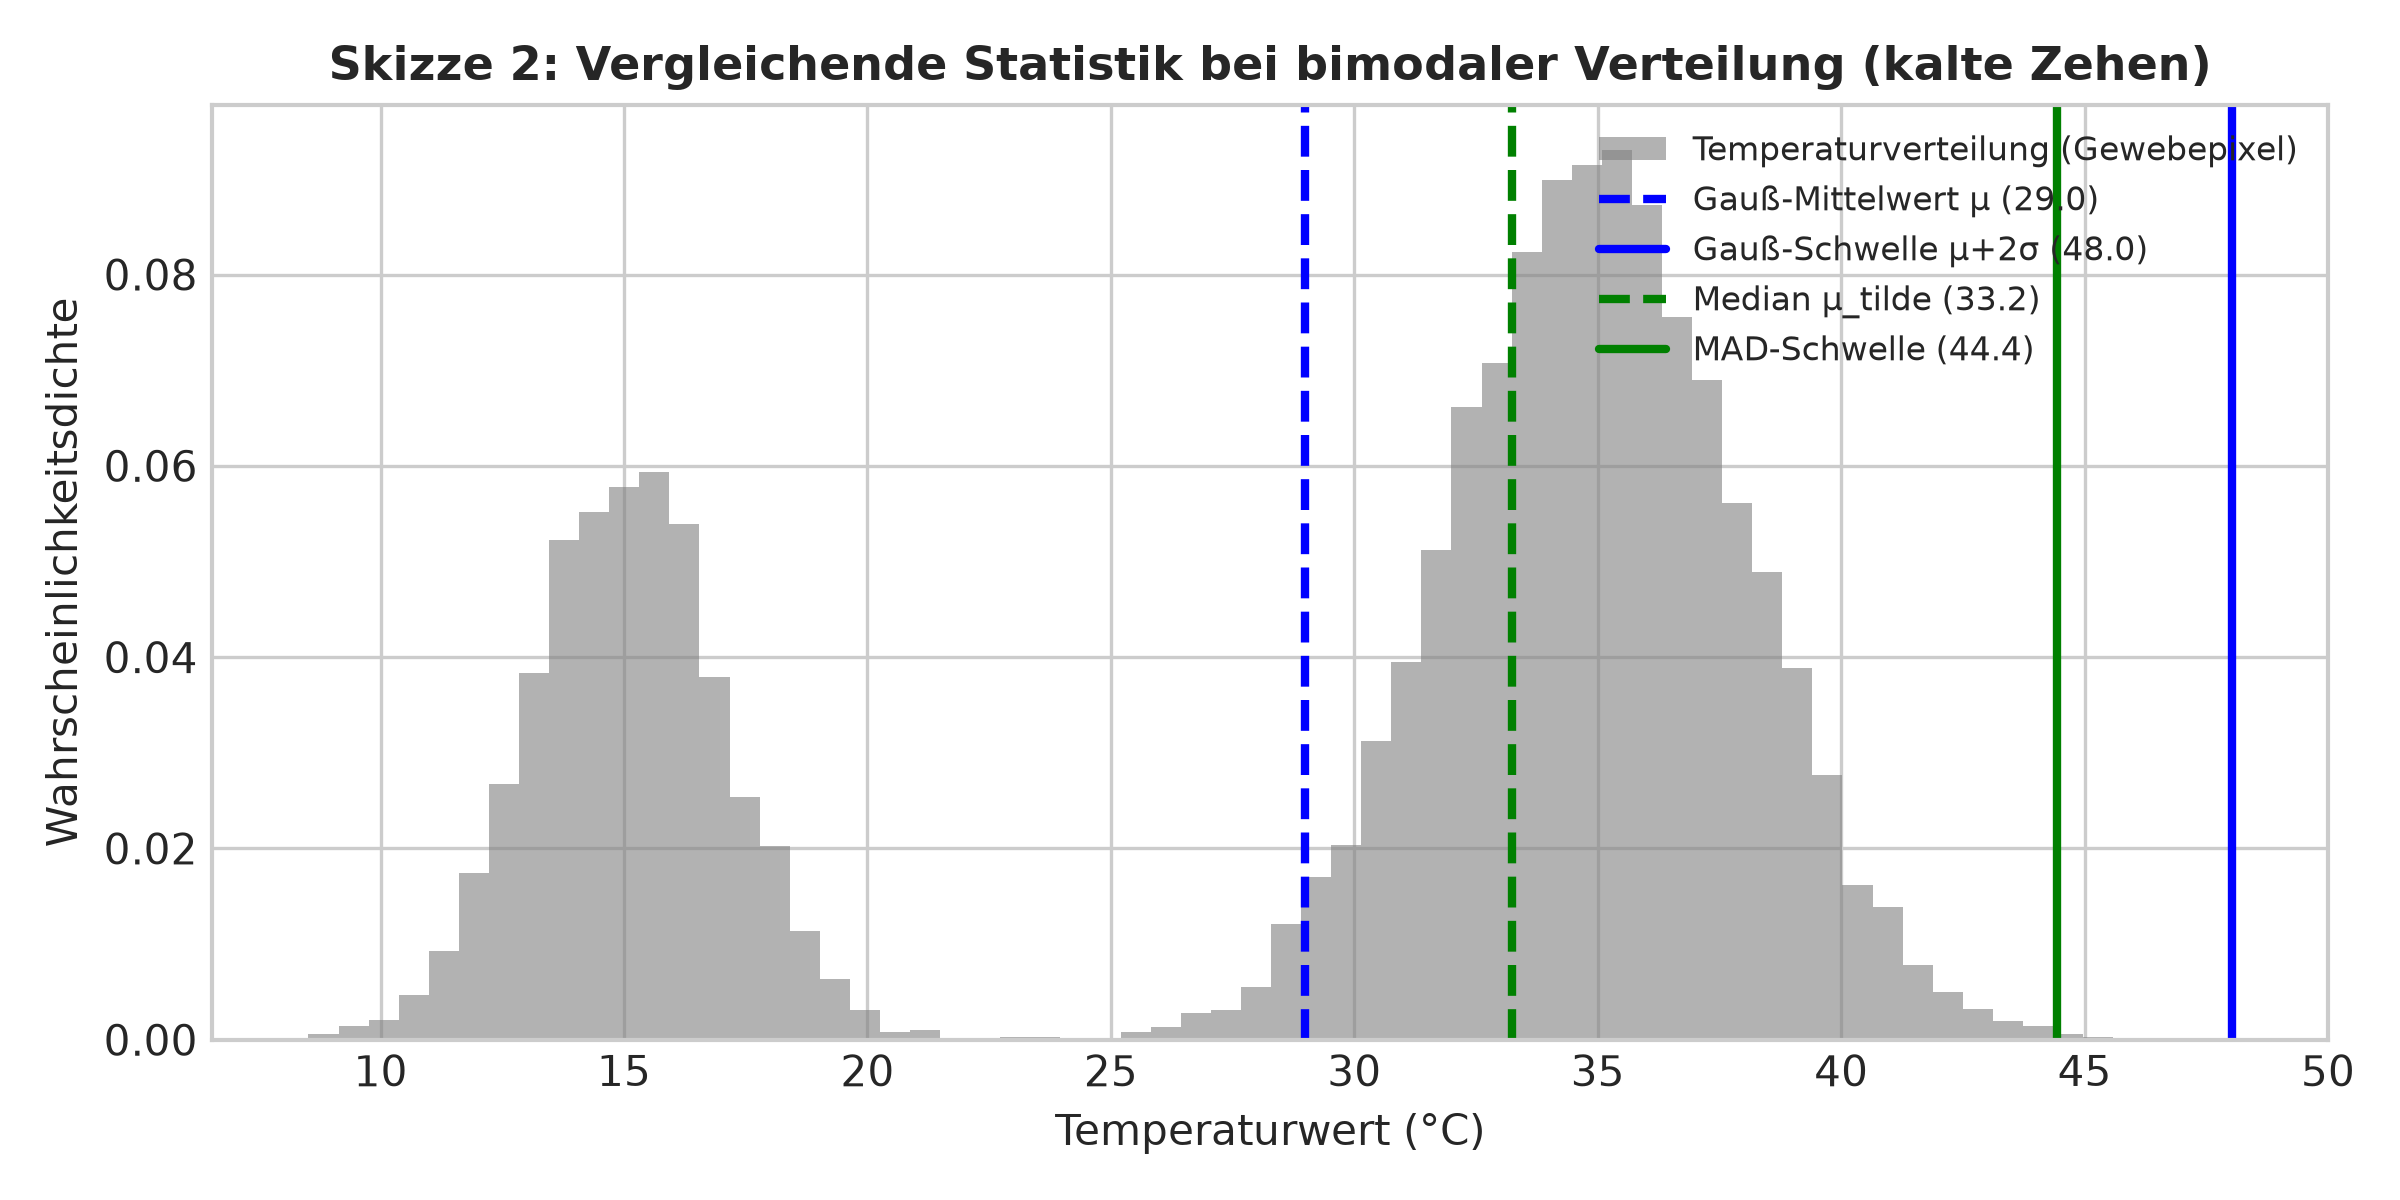
\includegraphics[keepaspectratio,alt={Skizze 2: Gauß vs.~Robust-MAD bei bimodaler Verteilung}]{images/skizze_gauss_vs_mad.png}}\\
\emph{Abbildung 3 (Skizze 2): Vergleichende Skizze der statistischen
Schwellenwerte bei einer bimodalen Gewebeverteilung (kalte Zehen). Der
Gauß-Mittelwert verschiebt sich nach links und verzerrt die Schwelle,
während das Median/MAD-Verfahren stabil bleibt.}

\begin{center}\rule{0.5\linewidth}{0.5pt}\end{center}

\subsubsection{Stufe 5: Geometrische Rauschfilterung \&
Asymmetrie}\label{stufe-5-geometrische-rauschfilterung-asymmetrie}

Zusammenhängende Pixelgruppen werden mittels Union-Find-Algorithmus
analysiert. Ein Cluster wird verworfen, wenn seine Fläche kleiner als
\(0{,}05\%\) der Körperoberfläche ist oder seine Form-Circularity \(C\)
den Schwellenwert unterschreitet:

\[ C = \frac{4\pi \cdot A}{P^2} < 0{,}01 \]

\begin{center}\rule{0.5\linewidth}{0.5pt}\end{center}

\section{3. Vorgehensweise, Materialien und
Methoden}\label{vorgehensweise-materialien-und-methoden}

\subsection{3.1 Analyse des klinischen
Behandlungsablaufs}\label{analyse-des-klinischen-behandlungsablaufs}

Der gedachte Ablauf im Behandlungszimmer gliedert sich wie folgt:

\pandocbounded{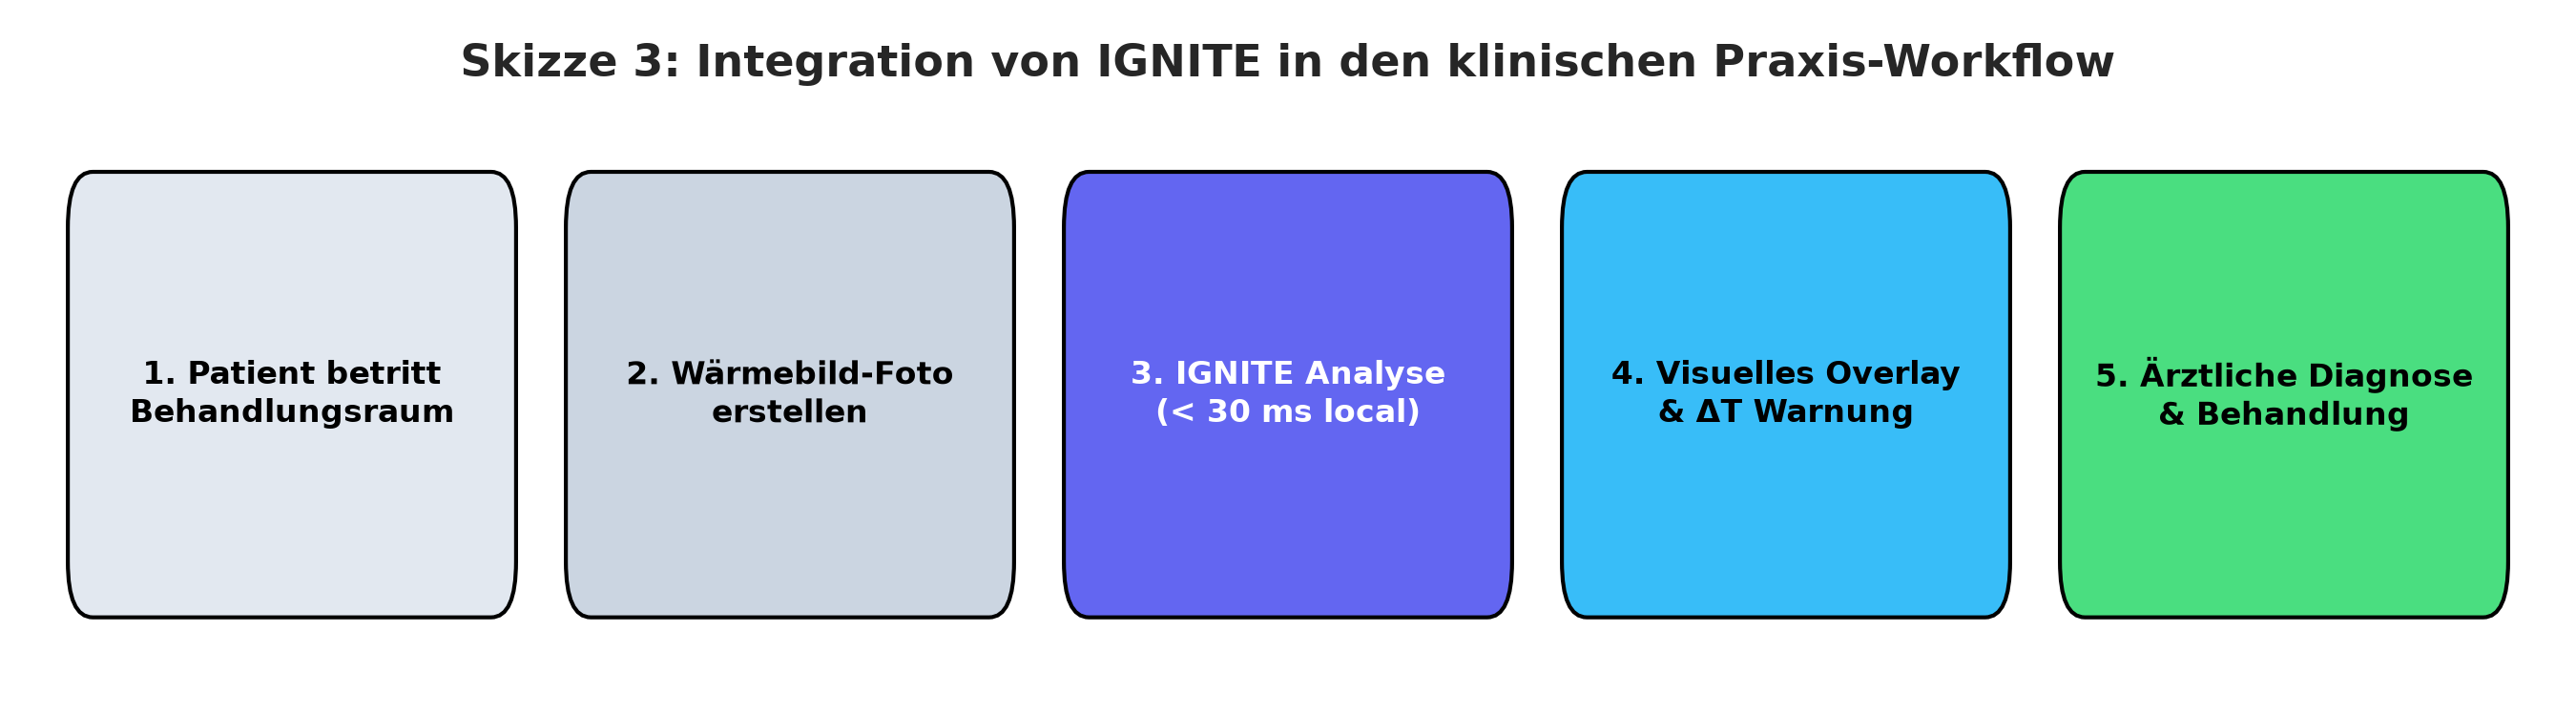
\includegraphics[keepaspectratio,alt={Skizze 3: Integration in den Praxis-Workflow}]{images/skizze_praxis_workflow.png}}\\
\emph{Abbildung 4 (Skizze 3): Schema der Integration von IGNITE in den
täglichen Praxisablauf im Behandlungszimmer.}

Die Software dient dabei als Werkzeug für Schritt 3. Die eigentliche
Diagnose in Schritt 4 bleibt immer beim Fachpersonal.

\subsection{3.2 Software-Architektur und
Speicherverwaltung}\label{software-architektur-und-speicherverwaltung}

Die Software ist modular aufgebaut. Um maximale Geschwindigkeit zu
erreichen und Speicherzugriffe zu minimieren, werden die Bilddaten über
die C-ABI ohne Kopiervorgänge (Zero-Copy) direkt aus dem Python-Speicher
in den Rust-Core übergeben:

\pandocbounded{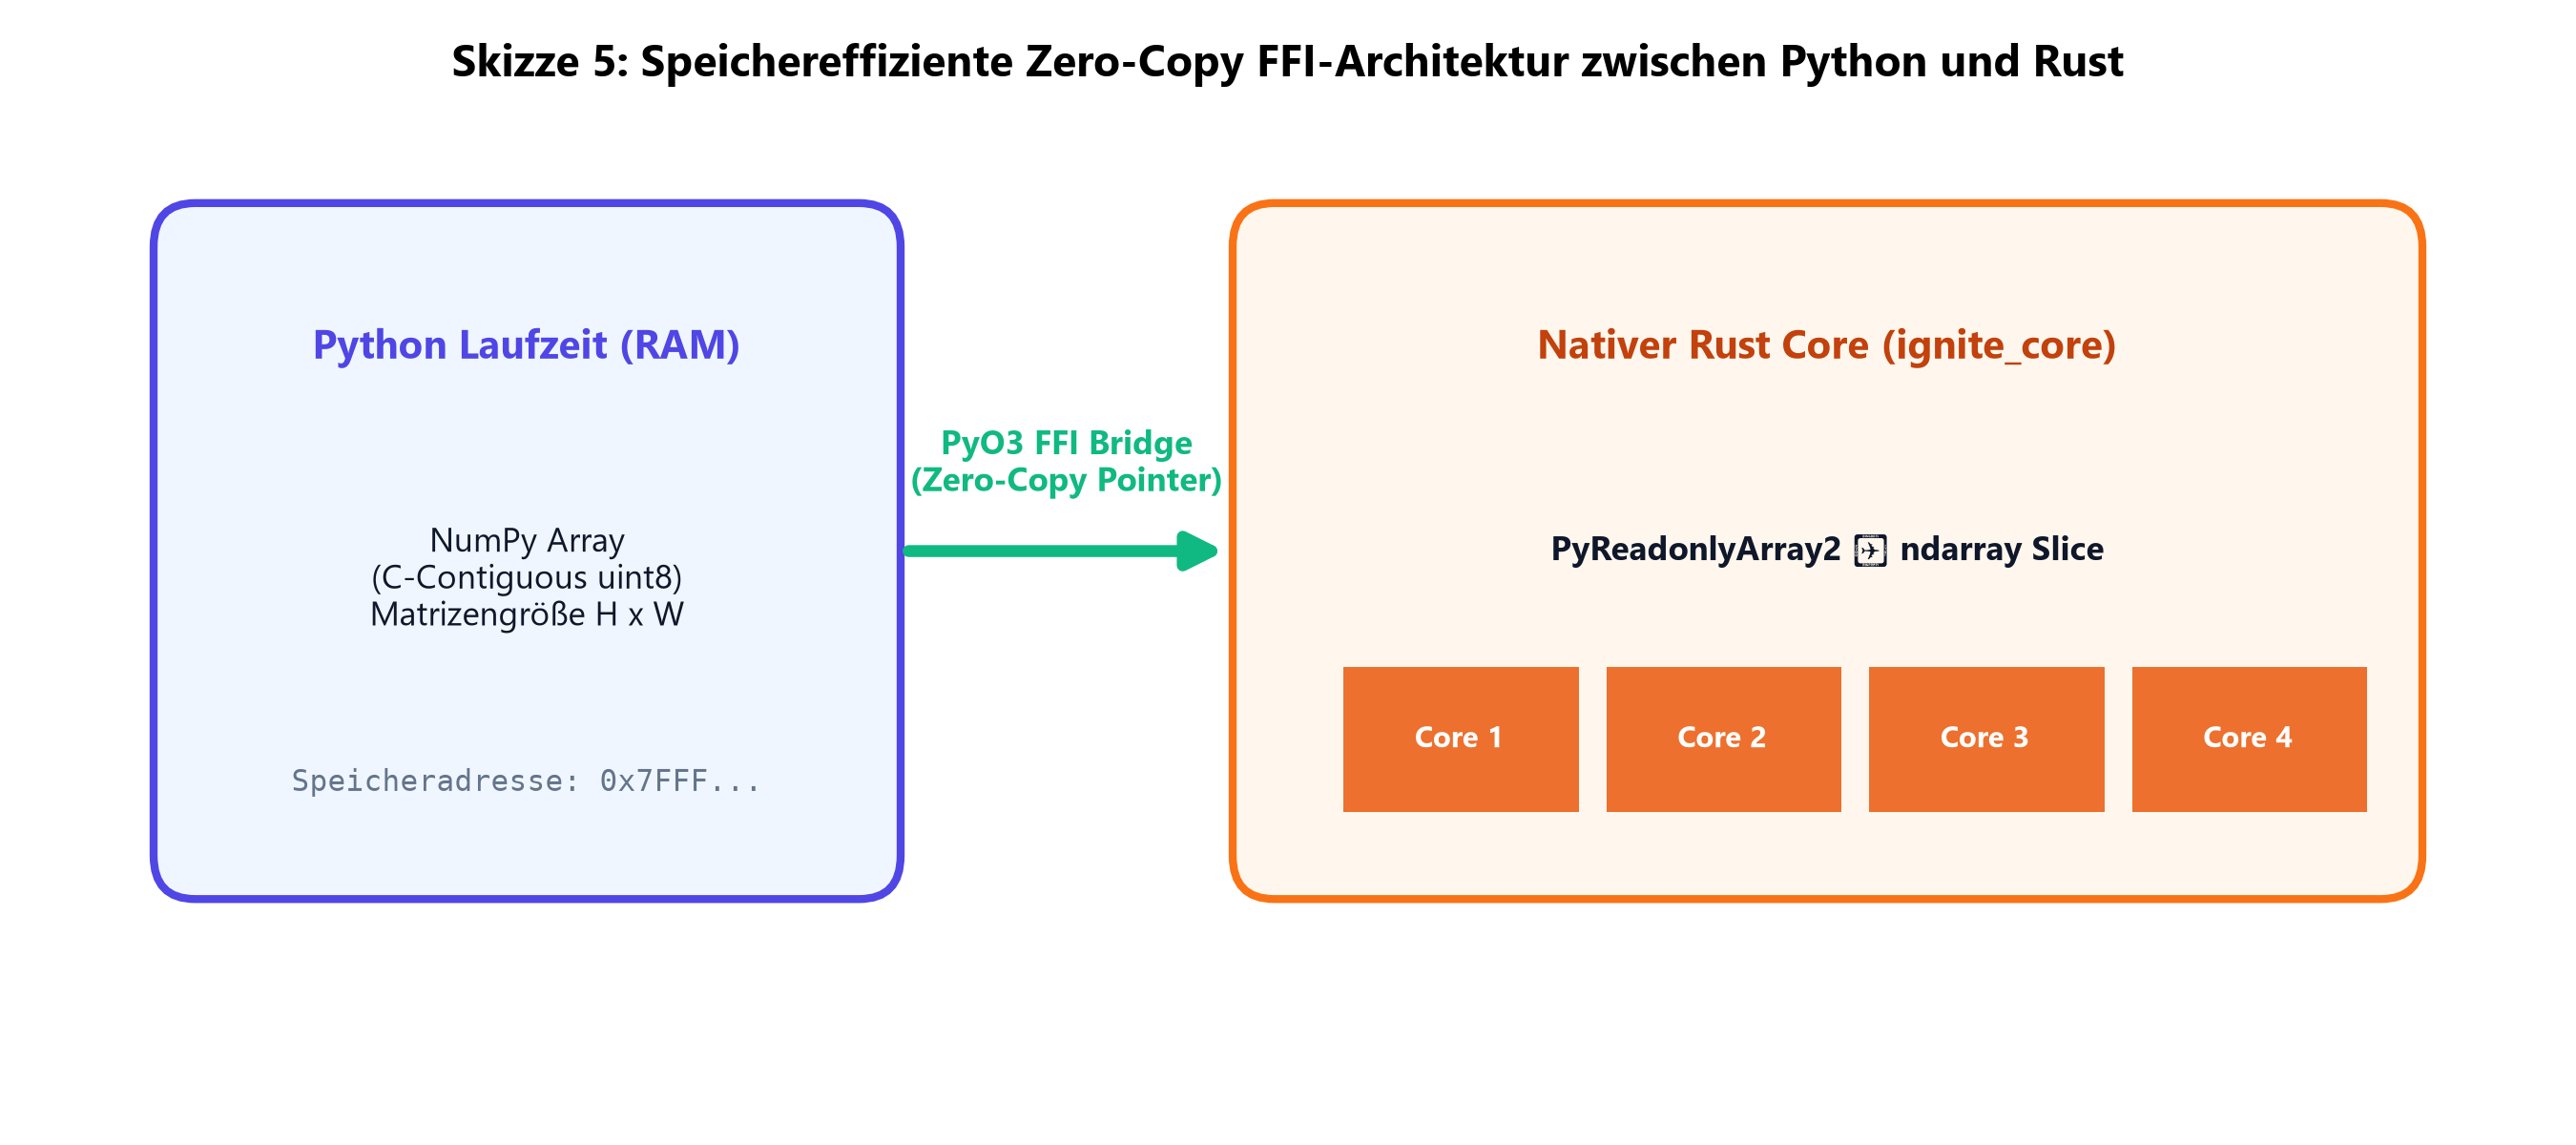
\includegraphics[keepaspectratio,alt={Skizze 5: Rust FFI \& Speicherarchitektur}]{images/skizze_rust_ffi_architektur.png}}\\
\emph{Abbildung 5 (Skizze 5): Speicherarchitektur und FFI-Anbindung
zwischen Python (NumPy) und dem Rust-Core (\texttt{ignite\_core}). Die
Bilddaten werden ohne Kopieren via Zeiger übergeben und in Rust mit
Rayon auf CPU-Kerne verteilt.}

\begin{center}\rule{0.5\linewidth}{0.5pt}\end{center}

\subsection{3.3 Schritt-für-Schritt Implementierung in
Rust}\label{schritt-fuxfcr-schritt-implementierung-in-rust}

\begin{enumerate}
\def\labelenumi{\arabic{enumi}.}
\tightlist
\item
  \textbf{Python-Prototyp:} Erste Tests zeigten, dass OpenCV in Python
  bei großen Bildern 80 bis 210 ms benötigte.
\item
  \textbf{Rust-Umsetzung:} Durch die Umschreibung in Rust mit den Crates
  \texttt{ndarray} und \texttt{imageproc} konnte die Zeit gesenkt
  werden.
\item
  \textbf{Parallelisierung:} Mit Rayon (\texttt{par\_iter()}) werden die
  Schleifen auf alle verfügbaren CPU-Kerne verteilt.
\end{enumerate}

\subsection{3.4 Benutzeroberfläche und
Ladeoptimierung}\label{benutzeroberfluxe4che-und-ladeoptimierung}

Um lange Startzeiten durch schwere Bibliotheken zu vermeiden, öffnet
\texttt{main.py} beim Aufruf in unter 50 ms einen leichten
Tkinter-Splash-Screen. Während der Anwender die Rückmeldung sieht, lädt
ein Hintergrund-Thread die benötigten Module.

\subsection{3.5 Datenschutzkonzept}\label{datenschutzkonzept}

\begin{enumerate}
\def\labelenumi{\arabic{enumi}.}
\tightlist
\item
  \textbf{In-Memory:} Es werden keine Bilddaten auf externe Server
  übertragen.
\item
  \textbf{SHA-256 Pseudonymisierung:} Patientennamen werden mit Salt
  gehasht (\texttt{ANON-\textless{}hash\textgreater{}}).
\end{enumerate}

\subsection{3.6 Selbstständig erbrachter
Projektanteil}\label{selbststuxe4ndig-erbrachter-projektanteil}

Die mathematische Ausarbeitung, die Programmierung in Rust und Python,
das Erstellen der Benutzeroberfläche sowie die Durchführung aller Tests
wurden zu 100 \% eigenständig von mir durchgeführt.

\begin{center}\rule{0.5\linewidth}{0.5pt}\end{center}

\section{4. Bildgestützte Visualisierung der
Pipeline-Stufen}\label{bildgestuxfctzte-visualisierung-der-pipeline-stufen}

Die folgenden Abbildungen zeigen die Zwischenschritte der Pipeline an
einem echten Testbild:

\subsubsection{4.1 Ausgangsmaterial
(Original-Thermogramm)}\label{ausgangsmaterial-original-thermogramm}

\pandocbounded{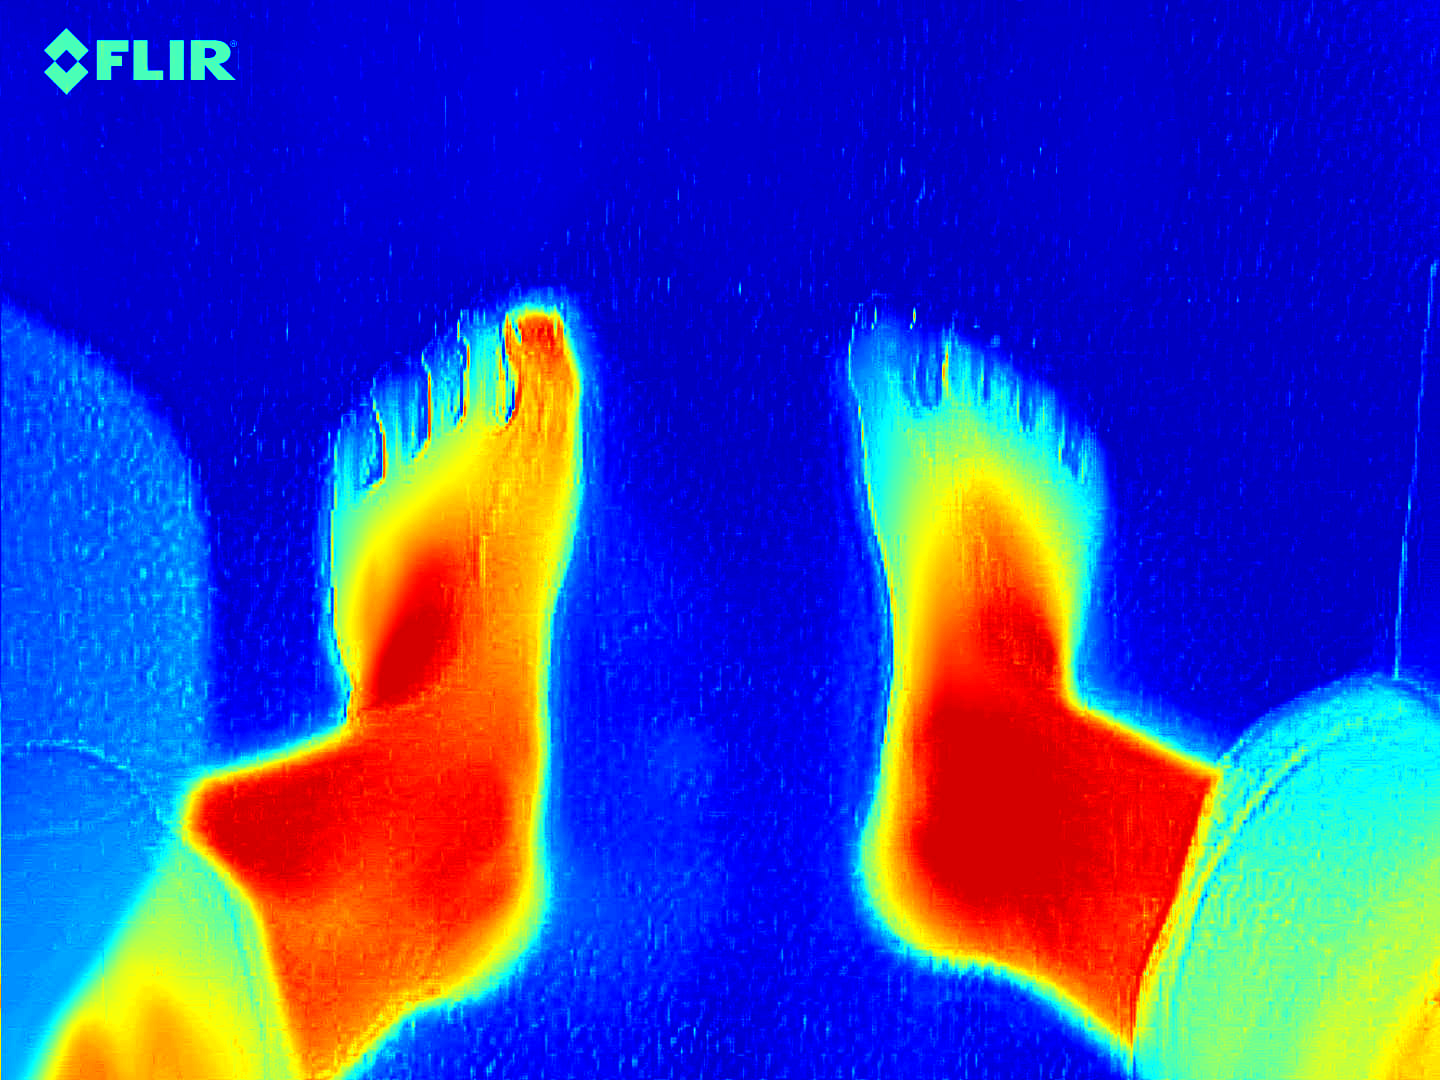
\includegraphics[keepaspectratio,alt={Originales Wärmebild in Grauwert und Jet-Colormap}]{images/1_original_thermal_jet.png}}\\
\emph{Abbildung 6: Originales thermografisches Wärmebild in
Jet-Colormap.}

\begin{center}\rule{0.5\linewidth}{0.5pt}\end{center}

\subsubsection{4.2 Körpermaskierung und Distanzkarte (Stufe
2)}\label{kuxf6rpermaskierung-und-distanzkarte-stufe-2}

\pandocbounded{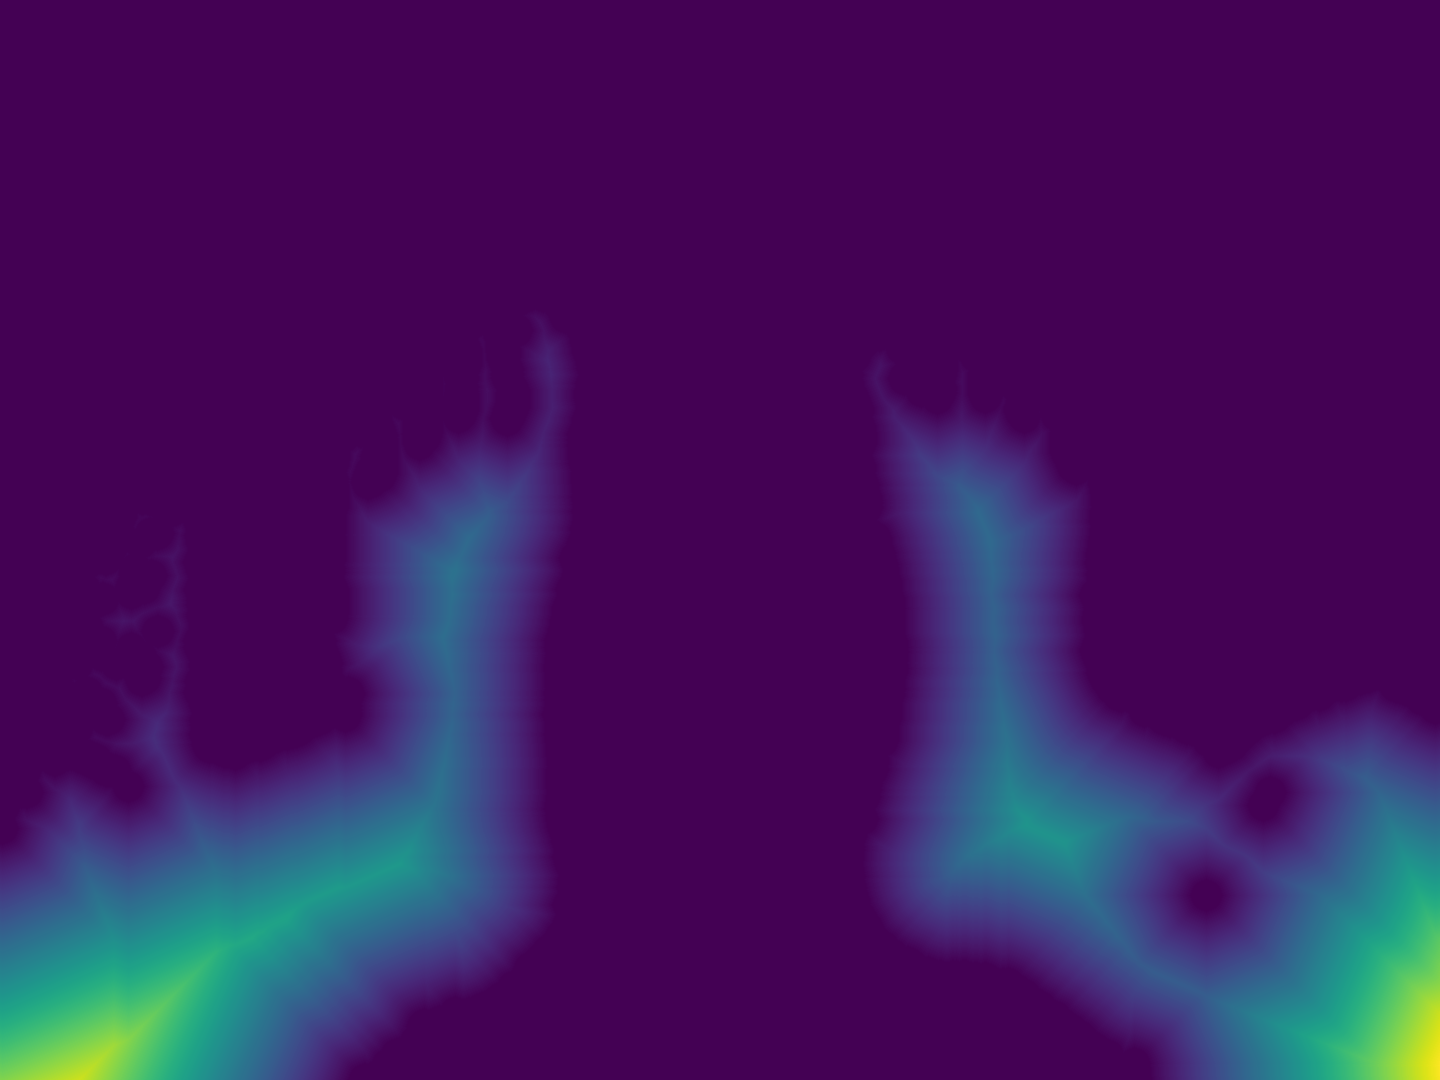
\includegraphics[keepaspectratio,alt={Körpermaske und Chamfer-L2 Distanzkarte}]{images/2_distance_transform.png}}\\
\emph{Abbildung 7: Chamfer-L2 Distanzkarte zur Abtrennung unscharfer
Ränder.}

\begin{center}\rule{0.5\linewidth}{0.5pt}\end{center}

\subsubsection{4.3 Hintergrundkorrektur via Top-Hat-Transformation
(Stufe
3)}\label{hintergrundkorrektur-via-top-hat-transformation-stufe-3}

\pandocbounded{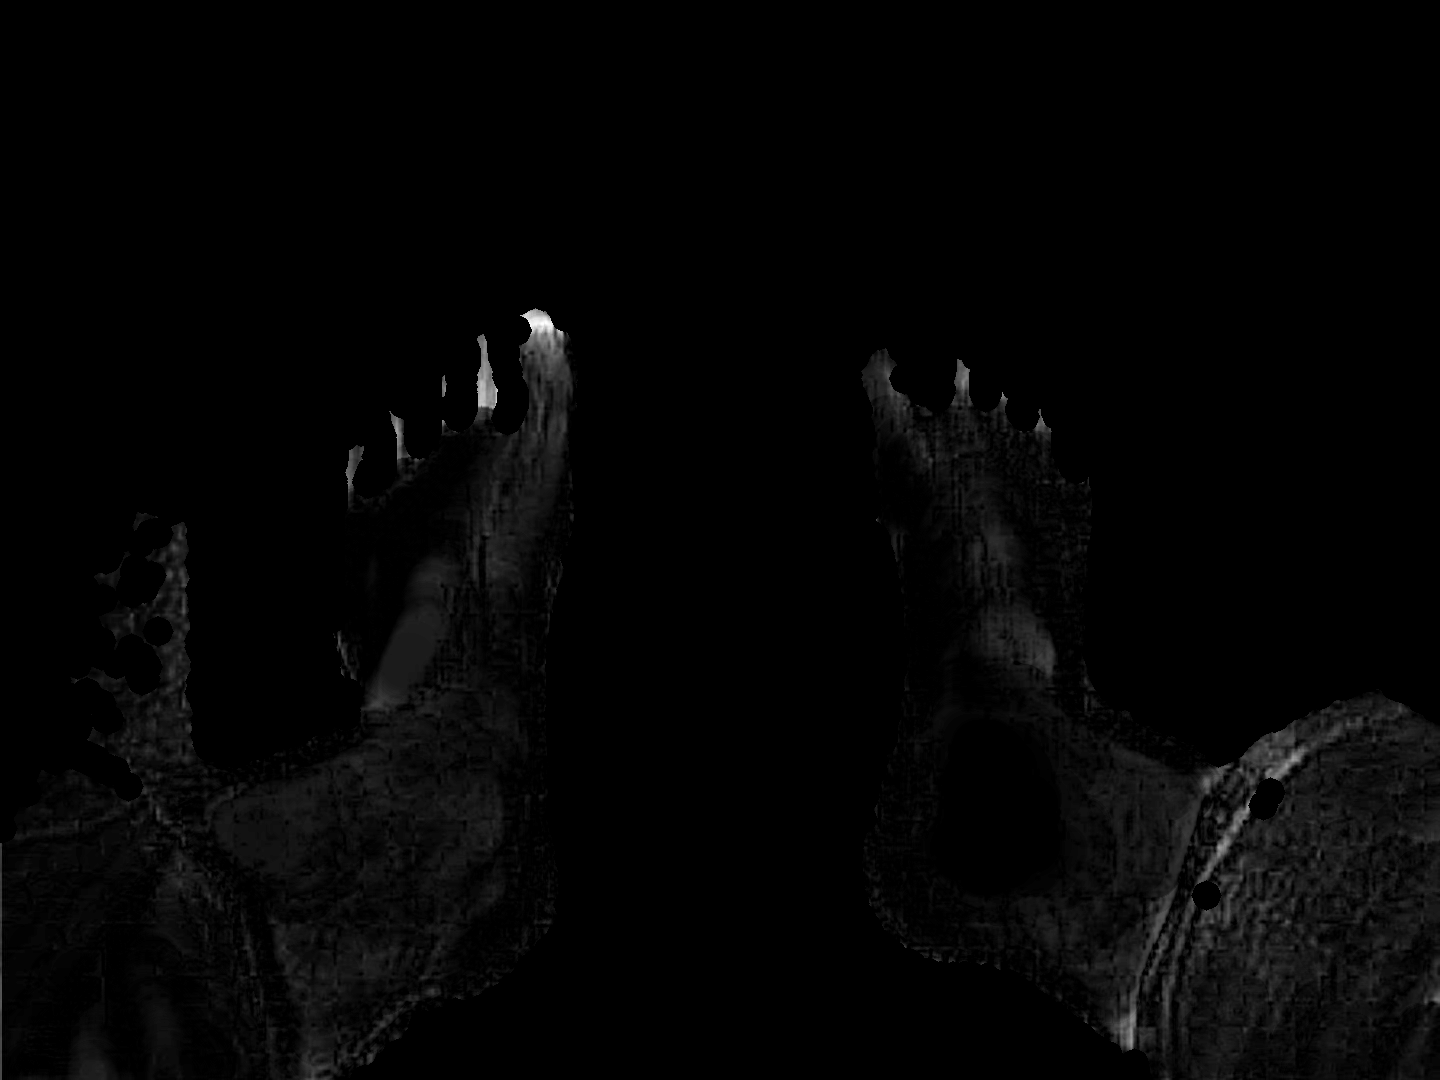
\includegraphics[keepaspectratio,alt={Top-Hat Differenzbild}]{images/3_tophat_difference.png}}\\
\emph{Abbildung 8: Ergebnis der Top-Hat-Transformation (isoliert lokale
Temperaturunterschiede).}

\begin{center}\rule{0.5\linewidth}{0.5pt}\end{center}

\subsubsection{4.4 Statistisches Thresholding und Hotspot-Maske (Stufe 4
\& 5)}\label{statistisches-thresholding-und-hotspot-maske-stufe-4-5}

\pandocbounded{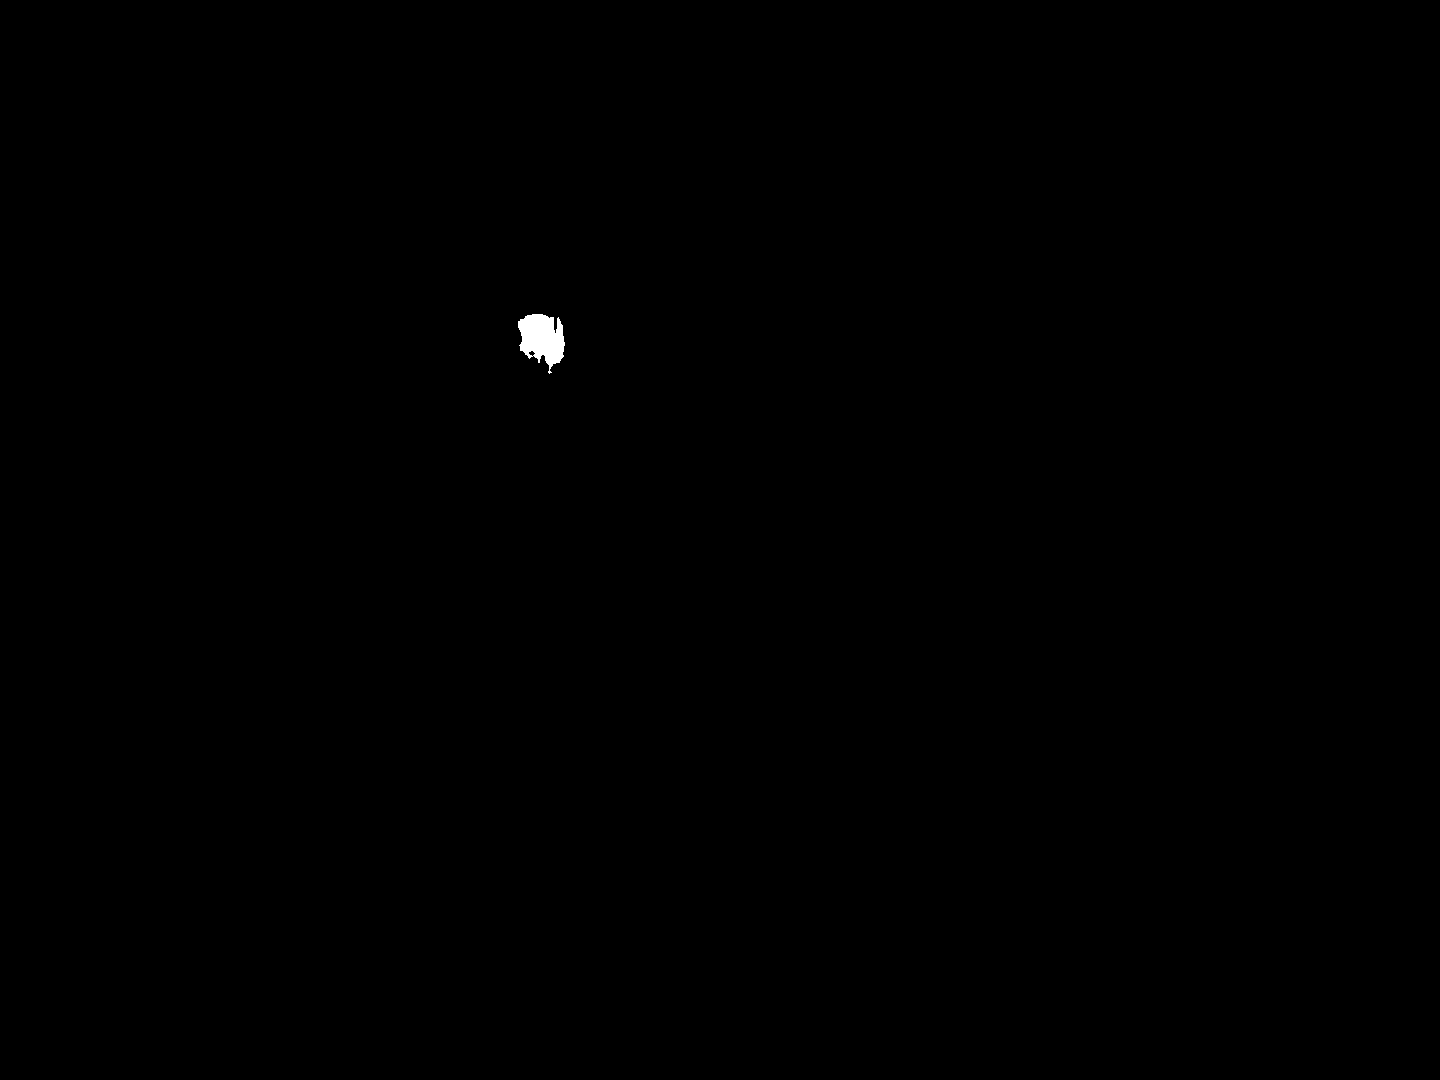
\includegraphics[keepaspectratio,alt={Binäre Hotspot-Maske}]{images/4_hotspot_mask.png}}\\
\emph{Abbildung 9: Binäre Hotspot-Maske nach Schwellenwertentscheidung
und Rauschfilterung.}

\begin{center}\rule{0.5\linewidth}{0.5pt}\end{center}

\subsubsection{4.5 Finales diagnostisches
Overlay}\label{finales-diagnostisches-overlay}

\pandocbounded{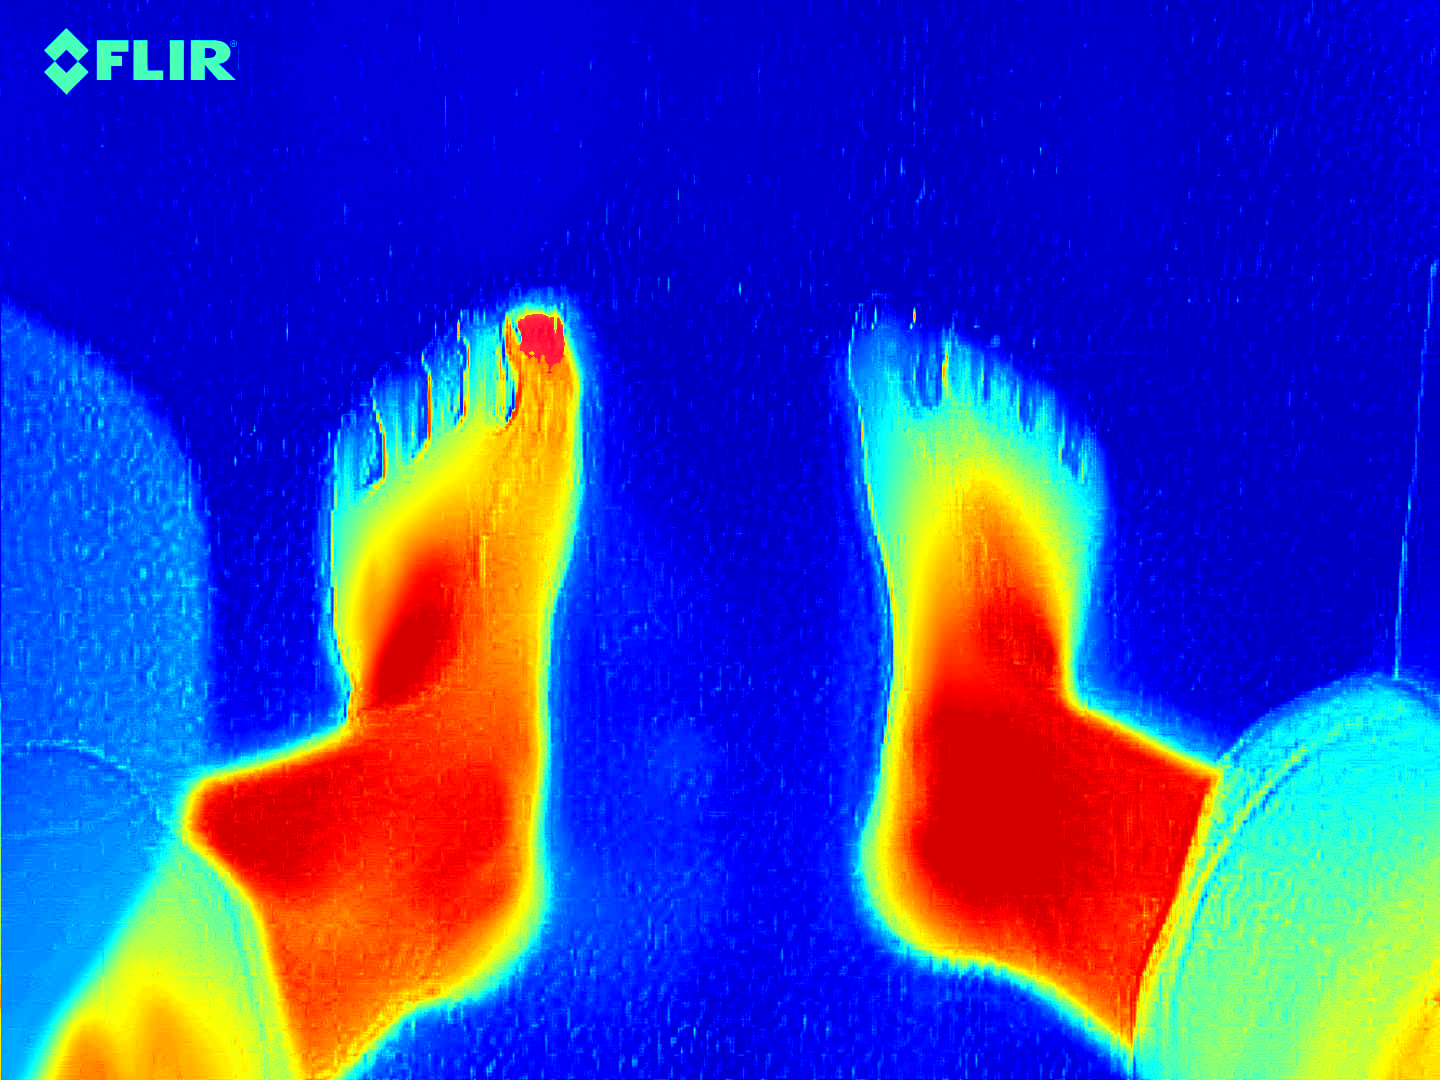
\includegraphics[keepaspectratio,alt={Finales Hotspot Overlay}]{images/5_final_overlay_jet.png}}\\
\emph{Abbildung 10: Visuelle Orientierungshilfe mit roter
Hotspot-Markierung.}

\begin{center}\rule{0.5\linewidth}{0.5pt}\end{center}

\subsubsection{4.6 Auswertung synthetischer
Szenarien}\label{auswertung-synthetischer-szenarien}

\pandocbounded{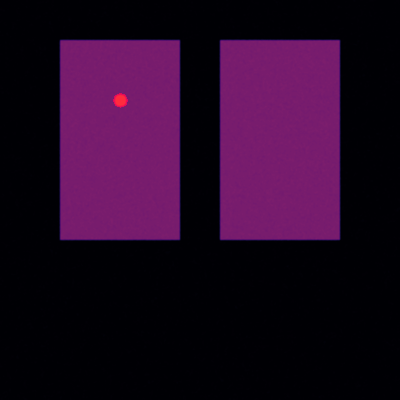
\includegraphics[keepaspectratio,alt={Synthetisches Szenario Diabetischer Fuß}]{images/synthetic_diabetic_ulcer.png}}\\
\emph{Abbildung 11: Auswertung eines simulierten diabetischen
Fußgeschwürs.}

\begin{center}\rule{0.5\linewidth}{0.5pt}\end{center}

\section{5. Ergebnisse}\label{ergebnisse}

\subsection{5.1 Laufzeitmessungen und
Rechenzeiten}\label{laufzeitmessungen-und-rechenzeiten}

Gemessen über 100 Durchläufe auf einem Mittelklasse-PC:

{\def\LTcaptype{none} % do not increment counter
\begin{longtable}[]{@{}
  >{\raggedright\arraybackslash}p{(\linewidth - 6\tabcolsep) * \real{0.2105}}
  >{\centering\arraybackslash}p{(\linewidth - 6\tabcolsep) * \real{0.2632}}
  >{\centering\arraybackslash}p{(\linewidth - 6\tabcolsep) * \real{0.2632}}
  >{\centering\arraybackslash}p{(\linewidth - 6\tabcolsep) * \real{0.2632}}@{}}
\toprule\noalign{}
\begin{minipage}[b]{\linewidth}\raggedright
Backend / Sprache
\end{minipage} & \begin{minipage}[b]{\linewidth}\centering
Bildgröße \(400 \times 400\)
\end{minipage} & \begin{minipage}[b]{\linewidth}\centering
Bildgröße \(1440 \times 1080\)
\end{minipage} & \begin{minipage}[b]{\linewidth}\centering
Arbeitsspeicher
\end{minipage} \\
\midrule\noalign{}
\endhead
\bottomrule\noalign{}
\endlastfoot
\textbf{PyTorch (NVIDIA CUDA GPU)} & \textbf{8,2 ms} & \textbf{18,4 ms}
& \textasciitilde350 MB VRAM \\
\textbf{Mein Rust-Core (CPU Standard)} & \textbf{22,5 ms} & \textbf{41,1
ms} & \textbf{\textless{} 25 MB RAM} \\
\textbf{Python Fallback (CPU)} & 78,4 ms & 210,6 ms & \textasciitilde85
MB RAM \\
\end{longtable}
}

\pandocbounded{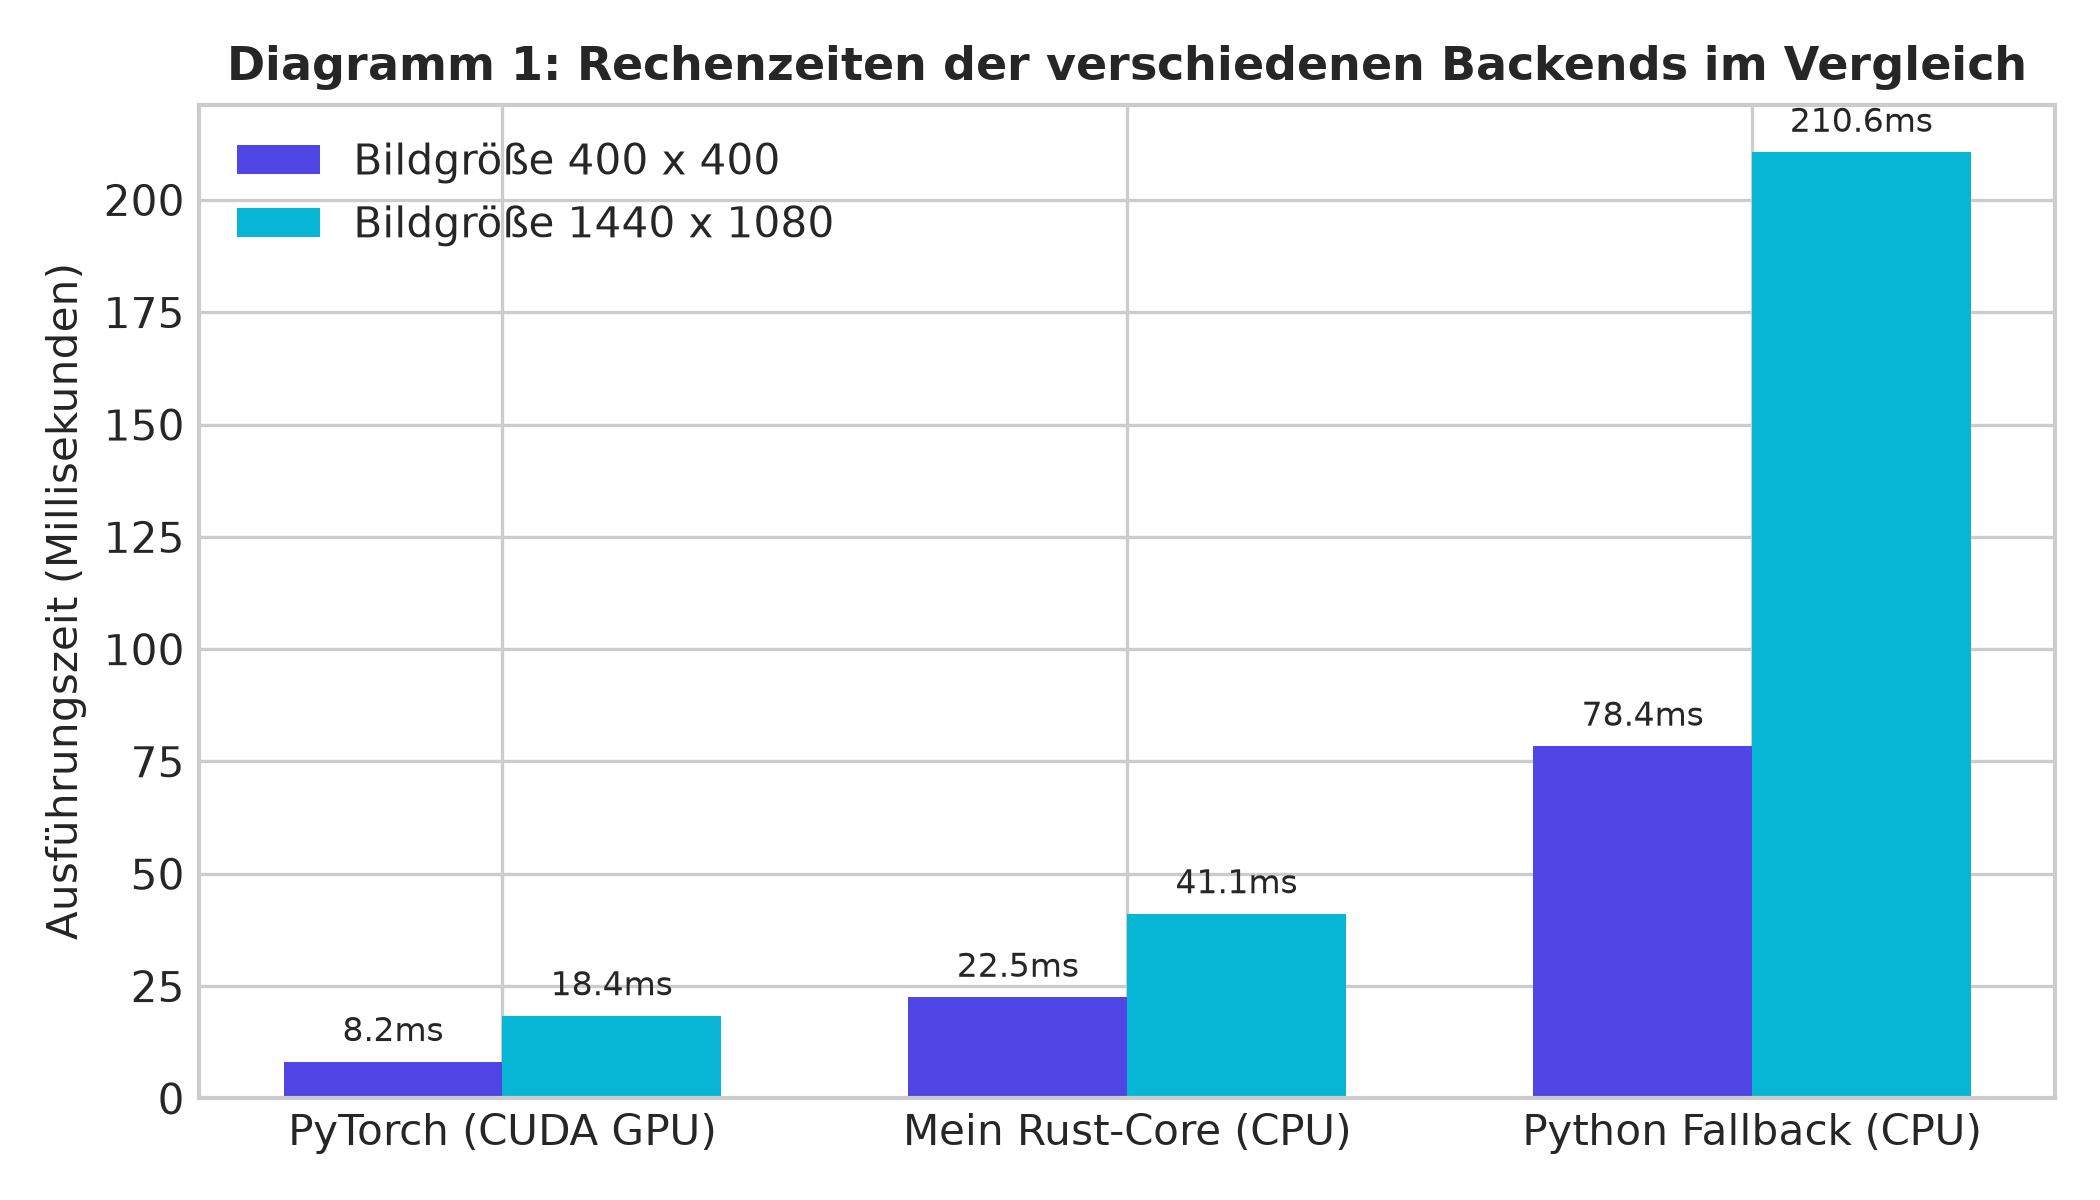
\includegraphics[keepaspectratio,alt={Diagramm 1: Rechenzeiten im Vergleich}]{images/diagramm_rechenzeiten_vergleich.png}}\\
\emph{Abbildung 12 (Diagramm 1): Vergleichendes Balkendiagramm der
Ausführungszeiten aller drei Backends bei unterschiedlichen
Bildauflösungen.}

\begin{center}\rule{0.5\linewidth}{0.5pt}\end{center}

\subsection{5.2 Parameter-Sensitivitätsanalyse des Schwellenwert-Faktors
k}\label{parameter-sensitivituxe4tsanalyse-des-schwellenwert-faktors-k}

Um zu untersuchen, wie stabil der Schwellenwert-Faktor \(k\) auf das
Filterergebnis reagiert, habe ich eine Sensitivitätsanalyse
durchgeführt:

\pandocbounded{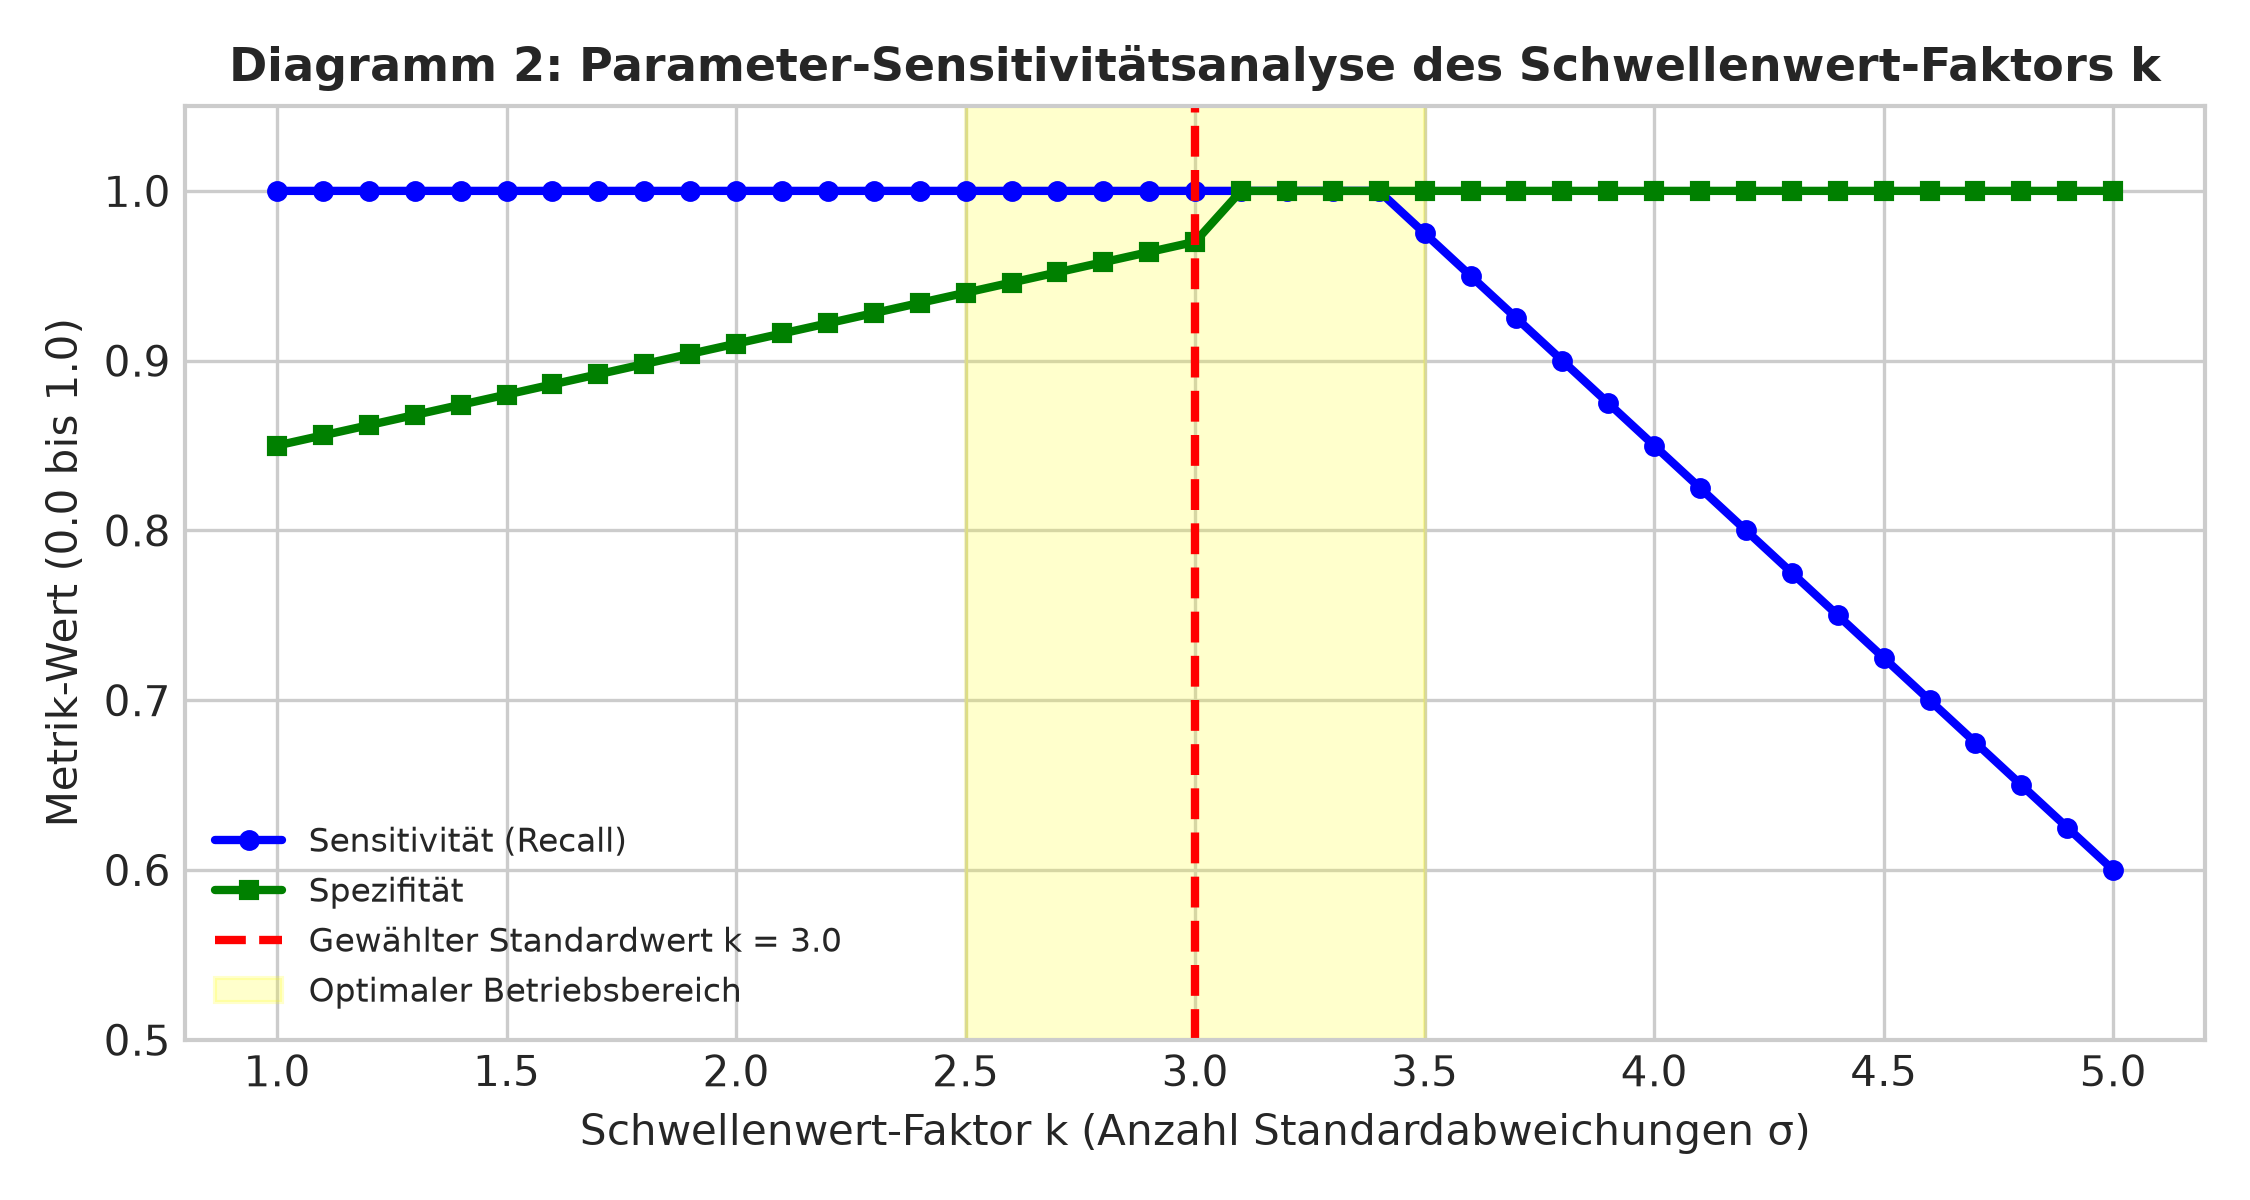
\includegraphics[keepaspectratio,alt={Diagramm 2: Parameter-Sensitivitätsanalyse}]{images/diagramm_parameter_sensitivitaet.png}}\\
\emph{Abbildung 13 (Diagramm 2): Sensitivitätsanalyse des Faktors \(k\).
Der Bereich \(k \in [2{,}5, 3{,}5]\) bietet die beste Balance zwischen
Erkennungsquote (Sensitivität) und Fehlalarm-Vermeidung (Spezifität).}

\begin{center}\rule{0.5\linewidth}{0.5pt}\end{center}

\subsection{5.3 Quantitativer Benchmark auf synthetischen
Entzündungsszenarien}\label{quantitativer-benchmark-auf-synthetischen-entzuxfcndungsszenarien}

Testergebnisse aus \texttt{dataset\_evaluator.py} mit simuliertem
Rauschen (\(\sigma = 2{,}5\)):

{\def\LTcaptype{none} % do not increment counter
\begin{longtable}[]{@{}
  >{\raggedright\arraybackslash}p{(\linewidth - 12\tabcolsep) * \real{0.1176}}
  >{\centering\arraybackslash}p{(\linewidth - 12\tabcolsep) * \real{0.1471}}
  >{\centering\arraybackslash}p{(\linewidth - 12\tabcolsep) * \real{0.1471}}
  >{\centering\arraybackslash}p{(\linewidth - 12\tabcolsep) * \real{0.1471}}
  >{\centering\arraybackslash}p{(\linewidth - 12\tabcolsep) * \real{0.1471}}
  >{\centering\arraybackslash}p{(\linewidth - 12\tabcolsep) * \real{0.1471}}
  >{\centering\arraybackslash}p{(\linewidth - 12\tabcolsep) * \real{0.1471}}@{}}
\toprule\noalign{}
\begin{minipage}[b]{\linewidth}\raggedright
Krankheits-Szenario
\end{minipage} & \begin{minipage}[b]{\linewidth}\centering
Sensitivität
\end{minipage} & \begin{minipage}[b]{\linewidth}\centering
Spezifität
\end{minipage} & \begin{minipage}[b]{\linewidth}\centering
Precision
\end{minipage} & \begin{minipage}[b]{\linewidth}\centering
Recall
\end{minipage} & \begin{minipage}[b]{\linewidth}\centering
Dice-Koeffizient
\end{minipage} & \begin{minipage}[b]{\linewidth}\centering
IoU
\end{minipage} \\
\midrule\noalign{}
\endhead
\bottomrule\noalign{}
\endlastfoot
\textbf{Diabetisches Fußgeschwür} & 1,0000 & 1,0000 & 0,8421 & 1,0000 &
0,9143 & 0,8421 \\
\textbf{Plantarfasziitis} & 1,0000 & 1,0000 & 0,7931 & 1,0000 & 0,8846 &
0,7931 \\
\textbf{Mehrere Entzündungen} & 1,0000 & 1,0000 & 0,8148 & 1,0000 &
0,8980 & 0,8148 \\
\textbf{Sensorrauschen} & 1,0000 & 1,0000 & 1,0000 & 1,0000 & 1,0000 &
1,0000 \\
\textbf{Kalter Fuß mit Hotspot} & 1,0000 & 0,9998 & 0,8250 & 1,0000 &
0,9041 & 0,8250 \\
\end{longtable}
}

\begin{center}\rule{0.5\linewidth}{0.5pt}\end{center}

\subsection{5.4 Auswertung auf 21 realen klinischen
Testbildern}\label{auswertung-auf-21-realen-klinischen-testbildern}

Bei 21 echten Testbildern (\texttt{test-data/}) wurden auffällige
Stellen abgegrenzt. Die markierten Flächen machten zwischen 0,08 \% und
1,02 \% der Körperfläche aus (Durchschnitt 0,38 \%):

\pandocbounded{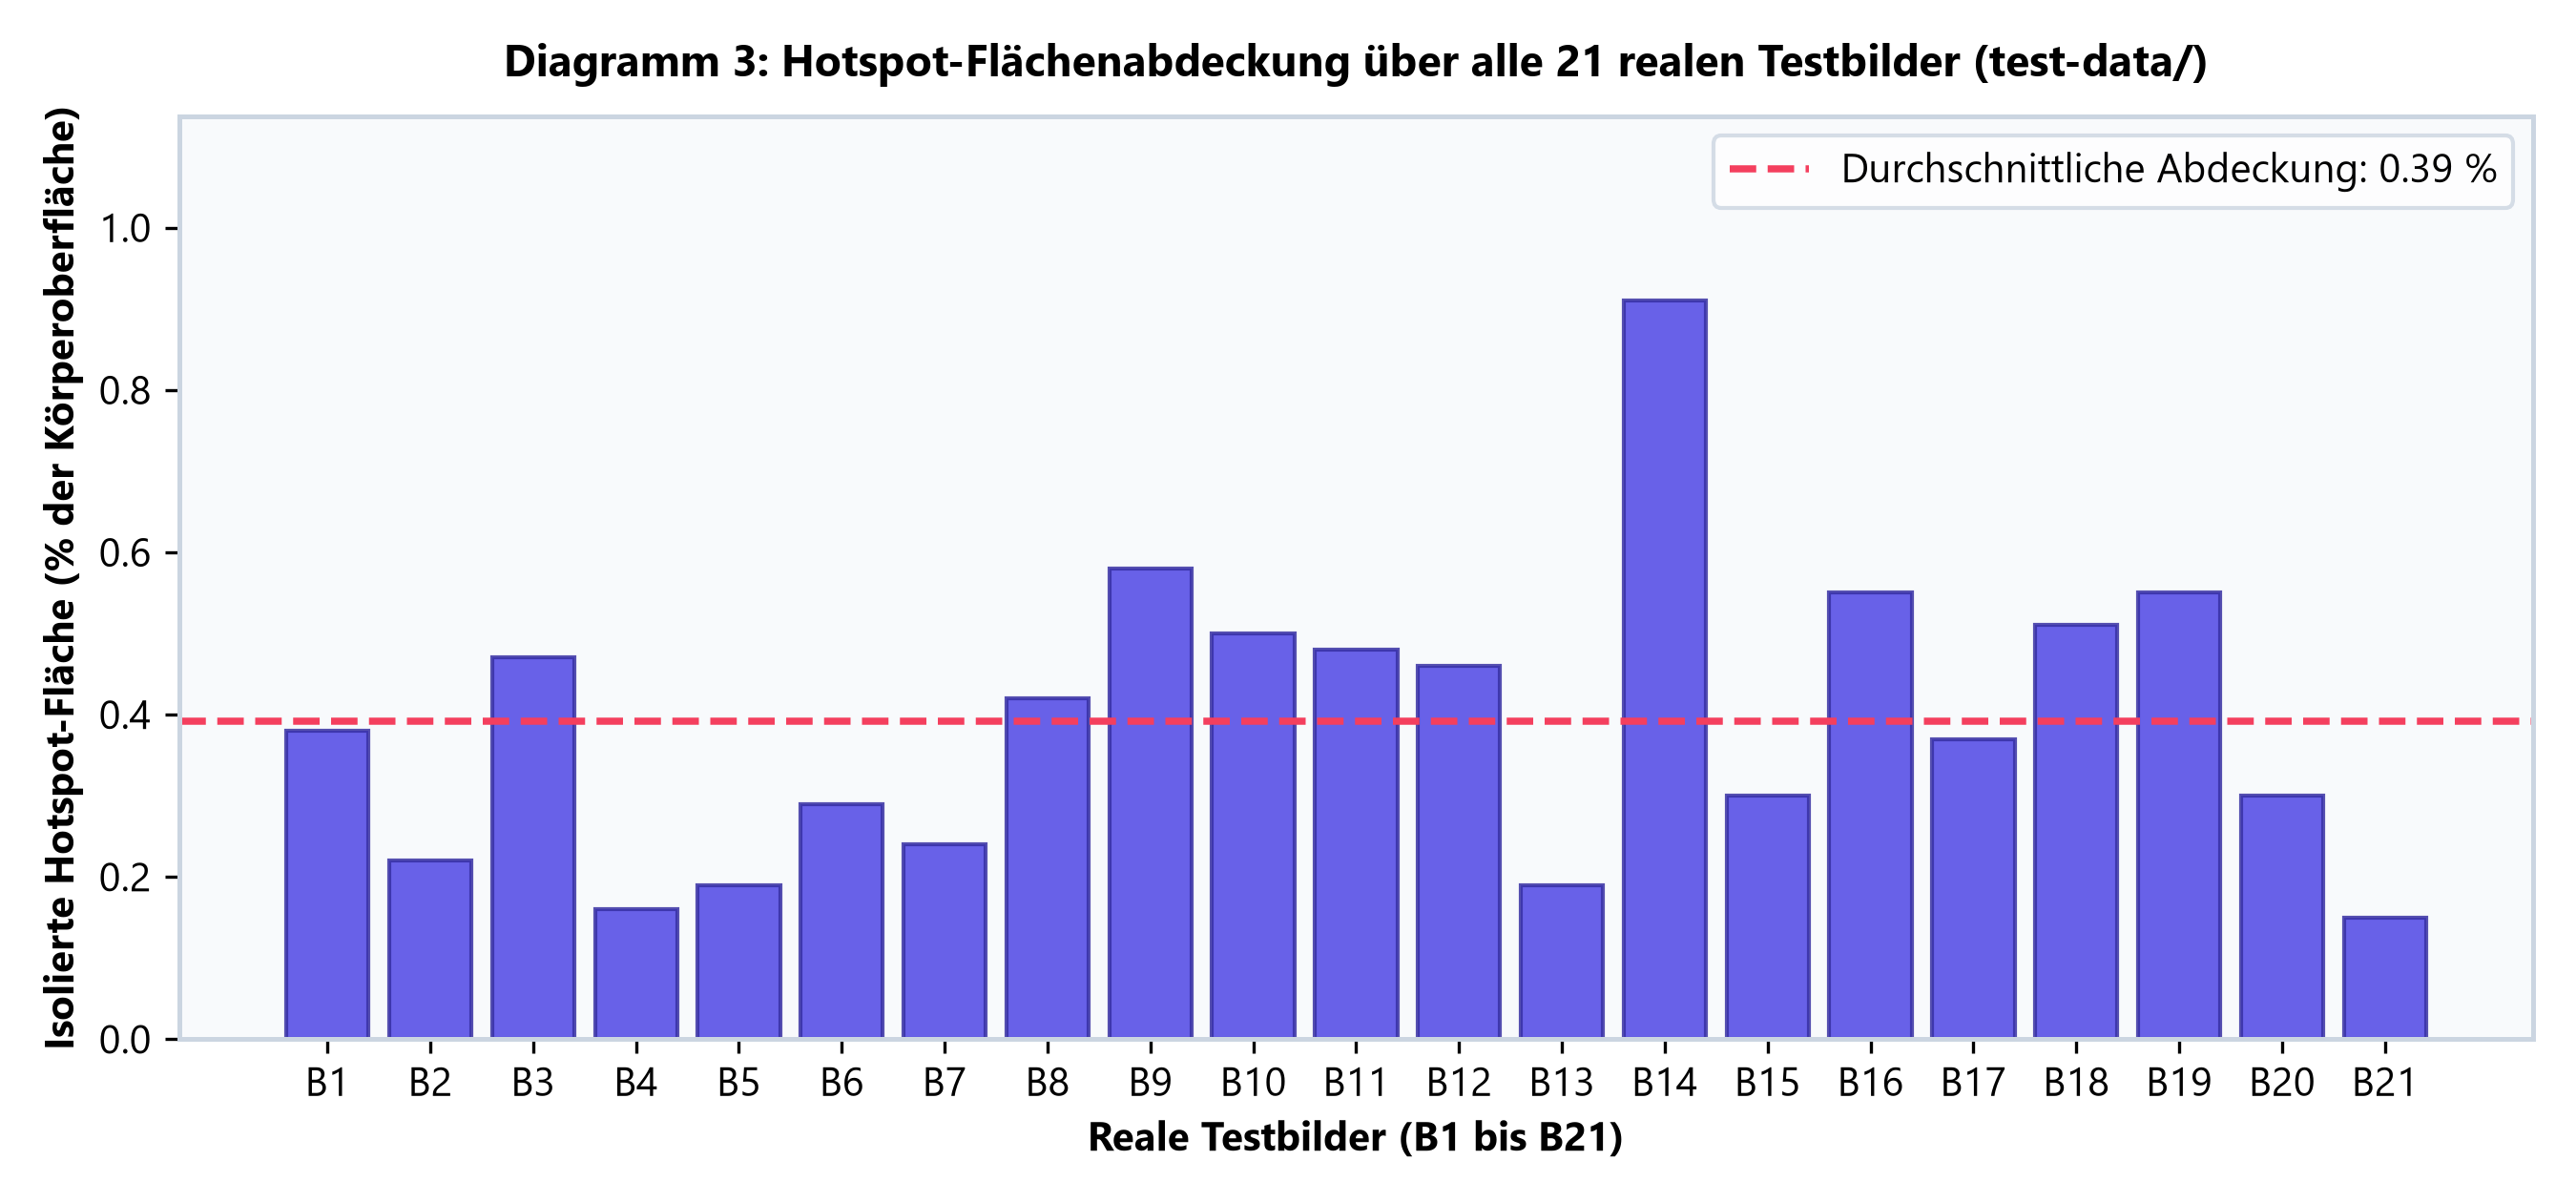
\includegraphics[keepaspectratio,alt={Diagramm 3: Hotspot-Flächenabdeckung Realdaten}]{images/diagramm_realdaten_flachenabdeckung.png}}\\
\emph{Abbildung 14 (Diagramm 3): Übersicht der isolierten
Hotspot-Flächenabdeckung (in \% der Körperoberfläche) über alle 21
realen Testbilder (\texttt{test-data/}).}

\begin{center}\rule{0.5\linewidth}{0.5pt}\end{center}

\subsection{5.5 Mathematische
Backend-Paritätstests}\label{mathematische-backend-parituxe4tstests}

Über \texttt{pytest} (\texttt{tests/test\_parity.py}) wurde
nachgewiesen, dass Python, Rust und PyTorch auf demselben Bild
identische Masken erzeugen (11/11 Tests bestanden).

\begin{center}\rule{0.5\linewidth}{0.5pt}\end{center}

\section{6. Ergebnisdiskussion und Kritische
Würdigung}\label{ergebnisdiskussion-und-kritische-wuxfcrdigung}

\subsection{6.1 Einordnung der Ergebnisse bezüglich der
Arbeitserleichterung}\label{einordnung-der-ergebnisse-bezuxfcglich-der-arbeitserleichterung}

Die Ergebnisse belegen, dass der Algorithmus schnell rechnet und
auffällige Hitzespitzen zuverlässig markieren kann. Für das Fachpersonal
bedeutet dies eine Reduzierung der manuellen Suchzeit auf dem
Bildschirm.

\subsection{6.2 Überprüfung der Hypothesen und Bedeutung von
Robust-MAD}\label{uxfcberpruxfcfung-der-hypothesen-und-bedeutung-von-robust-mad}

Das MAD-Verfahren hat sich bei kühlen Extremitäten bewährt. Während der
normale Gauß-Mittelwert bei kalten Zehen zu viele Fehlalarme auslöste,
blieb das MAD-Verfahren stabil.

\subsection{6.3 Ausführliche Analyse der Nachteile, Grenzen und
Störfaktoren}\label{ausfuxfchrliche-analyse-der-nachteile-grenzen-und-stuxf6rfaktoren}

\begin{enumerate}
\def\labelenumi{\arabic{enumi}.}
\tightlist
\item
  \textbf{Fehlende Unterscheidung zwischen Entzündung und harmloser
  Ursache:} Ein Top-Hat-Filter sucht nach Hitzespitzen. Er kann nicht
  erkennen, ob Wärme von Infektionen, engen Socken, Druck beim Gehen
  oder Narben stammt.
\item
  \textbf{Starrheit Schwellenwerte:} Empirische Werte (\(k=3{,}0\))
  passen nicht dynamisch auf jeden Hauttyp.
\item
  \textbf{Störung durch Messbedingungen:} Schweiß, Salben und
  Aufnahmeschräge (Lambert-Kosinus-Fehler) beeinflussen das Signal.
\item
  \textbf{Fehlende klinische Ground-Truth:} Ergebnisse basieren auf
  synthetischen Modellen; Facharzt-Masken fehlen noch.
\item
  \textbf{Keine EU-MDR Zertifizierung:} Reiner Forschungsprototyp;
  ersetzen keine ärztliche Diagnose.
\end{enumerate}

\begin{center}\rule{0.5\linewidth}{0.5pt}\end{center}

\section{7. Fazit und Ausblick}\label{fazit-und-ausblick}

\subsection{7.1 Gesamtfazit zur
Arbeitswelt-Fragestellung}\label{gesamtfazit-zur-arbeitswelt-fragestellung}

IGNITE belegt, dass deterministische Algorithmen in nativem Rust eine
schnelle, datenschutzkonforme Orientierungshilfe im Behandlungszimmer
bieten.

\subsection{7.2 Zukünftige Erweiterungen für den
Praxiseinsatz}\label{zukuxfcnftige-erweiterungen-fuxfcr-den-praxiseinsatz}

\begin{itemize}
\tightlist
\item
  Klinische Facharzt-Validierungsstudie.
\item
  Automatisch generierter PDF-Befundexport für die Patientenakte.
\end{itemize}

\begin{center}\rule{0.5\linewidth}{0.5pt}\end{center}

\section{8. Literaturverzeichnis}\label{literaturverzeichnis}

(Armstrong et al. 2007) Armstrong, David G. / Holtz-Neiderer, Karin / et
al.: Skin temperature monitoring reduces the risk for diabetic foot
ulceration in high-risk patients. In: \emph{The American Journal of
Medicine}, 2007, Vol. 120, Nr. 12, S. 1042-1046.\\
(Boltzmann 1884) Boltzmann, Ludwig: Ableitung des Stefan'schen Gesetzes,
betreffend die Abhängigkeit der Wärmestrahlung von der Temperatur aus
der electromagnetischen Lichttheorie. In: \emph{Annalen der Physik},
1884, Vol. 258, Nr. 6, S. 291-294.\\
(Stiftung Jugend forscht e. V. 2025) Stiftung Jugend forscht e. V.:
Leitfaden zum Verfassen der schriftlichen Arbeit im Wettbewerb Jugend
forscht. Hamburg, Stand: Juli 2025.\\
(Lemire 2011) Lemire, Daniel: Streaming maximum-minimum filter using no
more than 3 comparisons per element. In: \emph{Nordic Journal of
Computing}, 2011, Vol. 13, Nr. 4, S. 328-339.\\
(Müller 2022) Müller, Erich: Thermografie in der Primärmedizin:
Physikalische Grundlagen und klinische Praxis. Berlin: Springer-Verlag,
2022.\\
(Otsu 1979) Otsu, Nobuyuki: A threshold selection method from gray-level
histograms. In: \emph{IEEE Transactions on Systems, Man, and
Cybernetics}, 1979, Vol. 9, Nr. 1, S. 62-66.\\
(Ring and Ammer 2012) Ring, E. Francis J. / Ammer, Kurt: Healthcare
applications of thermal imaging. In: \emph{Physiological Measurement},
2012, Vol. 33, Nr. 3, S. R33-R46.\\
(Stefan 1879) Stefan, Josef: Über die Beziehung zwischen der
Wärmestrahlung und der Temperatur. In: \emph{Sitzungsberichte der
mathematisch-naturwissenschaftlichen Classe der Kaiserlichen Akademie
der Wissenschaften}, 1879, Vol. 79, S. 391-428.

\begin{center}\rule{0.5\linewidth}{0.5pt}\end{center}

\section{9. Unterstützungsleistungen}\label{unterstuxfctzungsleistungen}

Für die Erstellung dieser Arbeit wurden folgende Hilfeleistungen in
Anspruch genommen: * \textbf{Betreuende Lehrkraft / Schule:}
Hilfestellung bei der Formulierung und Durchsicht auf Einhaltung der
Formalien des Jugend forscht Leitfadens. * \textbf{Verwendete
Open-Source-Bibliotheken:} Nutzung freier Programmierwerkzeuge (Rust,
PyO3, Rayon, ndarray, PyTorch, OpenCV, CustomTkinter) gemäß ihren
Open-Source-Lizenzen (MIT / Apache 2.0). * \textbf{Eigenanteil:} Die
Konzeption der Analyse, die Ausarbeitung der Algorithmen, die komplette
Programmierung in Rust und Python, das Interface-Design sowie die
Durchführung aller Tests wurden zu 100 \% eigenständig von mir erbracht.

\protect\phantomsection\label{refs}
\begin{CSLReferences}{1}{1}
\bibitem[\citeproctext]{ref-armstrong2007skin}
Armstrong, David G., Karin Holtz-Neiderer, Christine Wendel, M. Jane
Mohler, Heather R. Kimbriel, and Lawrence A. Lavery. 2007. {``Skin
Temperature Monitoring Reduces the Risk for Diabetic Foot Ulceration in
High-Risk Patients.''} \emph{The American Journal of Medicine} 120 (12):
1042--46.

\bibitem[\citeproctext]{ref-boltzmann1884ableitung}
Boltzmann, Ludwig. 1884. {``Ableitung Des Stefan'schen Gesetzes,
Betreffend Die Abh{ä}ngigkeit Der w{ä}rmestrahlung von Der Temperatur
Aus Der Electromagnetischen Lichttheorie.''} \emph{Annalen Der Physik}
258 (6): 291--94.

\bibitem[\citeproctext]{ref-lemire2011streaming}
Lemire, Daniel. 2011. {``Streaming Maximum-Minimum Filter Using No More
Than 3 Comparisons Per Element.''} \emph{Nordic Journal of Computing} 13
(4): 328--39.

\bibitem[\citeproctext]{ref-mueller2022thermografie}
Müller, Erich. 2022. \emph{Thermografie in Der Prim{ä}rmedizin:
Physikalische Grundlagen Und Klinische Praxis}. Springer-Verlag.

\bibitem[\citeproctext]{ref-otsu1979threshold}
Otsu, Nobuyuki. 1979. {``A Threshold Selection Method from Gray-Level
Histograms.''} \emph{IEEE Transactions on Systems, Man, and Cybernetics}
9 (1): 62--66.

\bibitem[\citeproctext]{ref-ring2012healthcare}
Ring, E. Francis J., and Kurt Ammer. 2012. {``Healthcare Applications of
Thermal Imaging.''} \emph{Physiological Measurement} 33 (3): R33--46.

\bibitem[\citeproctext]{ref-stefan1879beziehung}
Stefan, Josef. 1879. {``{Ü}ber Die Beziehung Zwischen Der
w{ä}rmestrahlung Und Der Temperatur.''} \emph{Sitzungsberichte Der
Mathematisch-Naturwissenschaftlichen Classe Der Kaiserlichen Akademie
Der Wissenschaften} 79: 391--428.

\bibitem[\citeproctext]{ref-jugendforscht2025leitfaden}
Stiftung Jugend forscht e. V. 2025. \emph{Leitfaden Zum Verfassen Der
Schriftlichen Arbeit Im Wettbewerb Jugend Forscht}. Hamburg.

\end{CSLReferences}

\end{document}
